\documentclass[letterpaper,onecolumn,10pt,journal,final]{IEEEtran}

\usepackage{latexsym}


\usepackage[spanish,es-tabla]{babel}

\usepackage{amsmath}

\makeatletter
\newcommand\xleftrightarrow[2][]{%
  \ext@arrow 9999{\longleftrightarrowfill@}{#1}{#2}}
\newcommand\longleftrightarrowfill@{%
  \arrowfill@\leftarrow\relbar\rightarrow}
\makeatother

\usepackage{amsfonts}
\usepackage{subfigure}
\usepackage{psfrag}
\usepackage{colortbl}
\usepackage{color}
\usepackage[sectionbib]{chapterbib}
\usepackage{afterpage}
\usepackage{booktabs}

\usepackage{graphicx}
\usepackage{url}
\usepackage{amsmath}
\interdisplaylinepenalty=2500
\usepackage[english]{babel}
%\usepackage{array,booktabs,arydshln,xcolor}
\usepackage{flushend}
\hyphenation{industrial electronics IEEEtran}
\usepackage[font=footnotesize,caption=false,farskip=0mm,captionskip=0mm,nearskip=0mm]{subfig}
\usepackage{cite}
\usepackage{amsmath}
\usepackage{array}
\usepackage{graphicx}
\usepackage{latexsym}
\usepackage{psfrag}
\usepackage{color}
\usepackage{multirow}
\usepackage{stfloats}
\usepackage{enumerate}
% Paquetes adicionales para insertar código con formato m-file de MATLAB
\usepackage{listings}   % Permite incorporar código con diferentes formatos
\usepackage{float}
%usepackage{caption}
\usepackage[font=bf]{caption}
% falta cambiar el font size de caption  a 9pt
\usepackage[dvips]{graphicx}
\usepackage[framed,numbered,final]{mcode}% Configura listings para que el resultado se vea igual al editor de MATLAB
\usepackage{xcolor}
\usepackage{textcomp}

%\usepackage [latin1]{inputenc}
%\renewcommand\lstlistingname{Code}% Cambia el nombre del objeto listings

%ejemplo matlab code:

%\begin{lstlisting}[frame=single]
%a = 15;				% Por defecto es tipo 'double'
%b = uint8(a);		
%c = int16(32767);
%\end{lstlisting}

\parskip 0pt

\usepackage{lipsum}

\newcommand\blfootnote[1]{%
  \begingroup
  \renewcommand\thefootnote{}\footnote{#1}%
  \addtocounter{footnote}{-1}%
  \endgroup
}

\begin{document}
\title{ELO 314 - Procesamiento Digital de Señales\\ Laboratorio 5: Análisis y Compresión de Voz en MatLab}

\author{\textbf{Preparado por}
\vspace{1 mm}Juan Aguilera e-mail: Juan.Aguileraca@sansano.usm.cl \\
            Cristóbal Huidobro e-mail: 
cristobal.huidobro@sansano.usm.cl}

\maketitle

\vspace{-1 cm}

%\setcounter{section}{0}
%%%%%%%%%%%%%%%%%%%%%%%%%%%%%%%%%%%%%%%%%%%%%%%%%%%%%%%%%%%%%%%%%%%%%%%%%%%%%%%%%
%
%-----I PREDICCION´ LINEAL Y S´INTESIS DE VOCALES---------------------------------%
%
%%%%%%%%%%%%%%%%%%%%%%%%%%%%%%%%%%%%%%%%%%%%%%%%%%%%%%%%%%%%%%%%%%%%%%%%%%%%%%%%%
\section{Predicción Lineal y Síntesis de vocales}
\begin{enumerate}[1)]
    \item %1)------------------------------------------------------------------% 
%
Se genera la función siguiente.
%
\begin{lstlisting}
function X = exciteV (N, Np)
  for i=1:1:N
    if mod(i-1,Np) == 0
      X(i)=1;
    else
      X(i)=0;
    end
  end
 end
\end{lstlisting}
%
La cual se aplica de la siguiente manera para generar la señal con frecuencia fundamental de 100 Hz.
%
\begin{lstlisting}
fs=8000;
N=fs;
Np=80;
X = exciteV(N,Np);
\end{lstlisting}
%
La magnitud del espectro resultante se muestra en la Figura \ref{P1_1}. Se observa que efectivamente, la magnitud corresponden a pulsos separados por una frecuencia de $100~sps$. Al oír la señal se escucha un sonido con una frecuencia musical sostenida, levemente parecido a un instrumento de viento.
%
\begin{figure}[H]
\centering
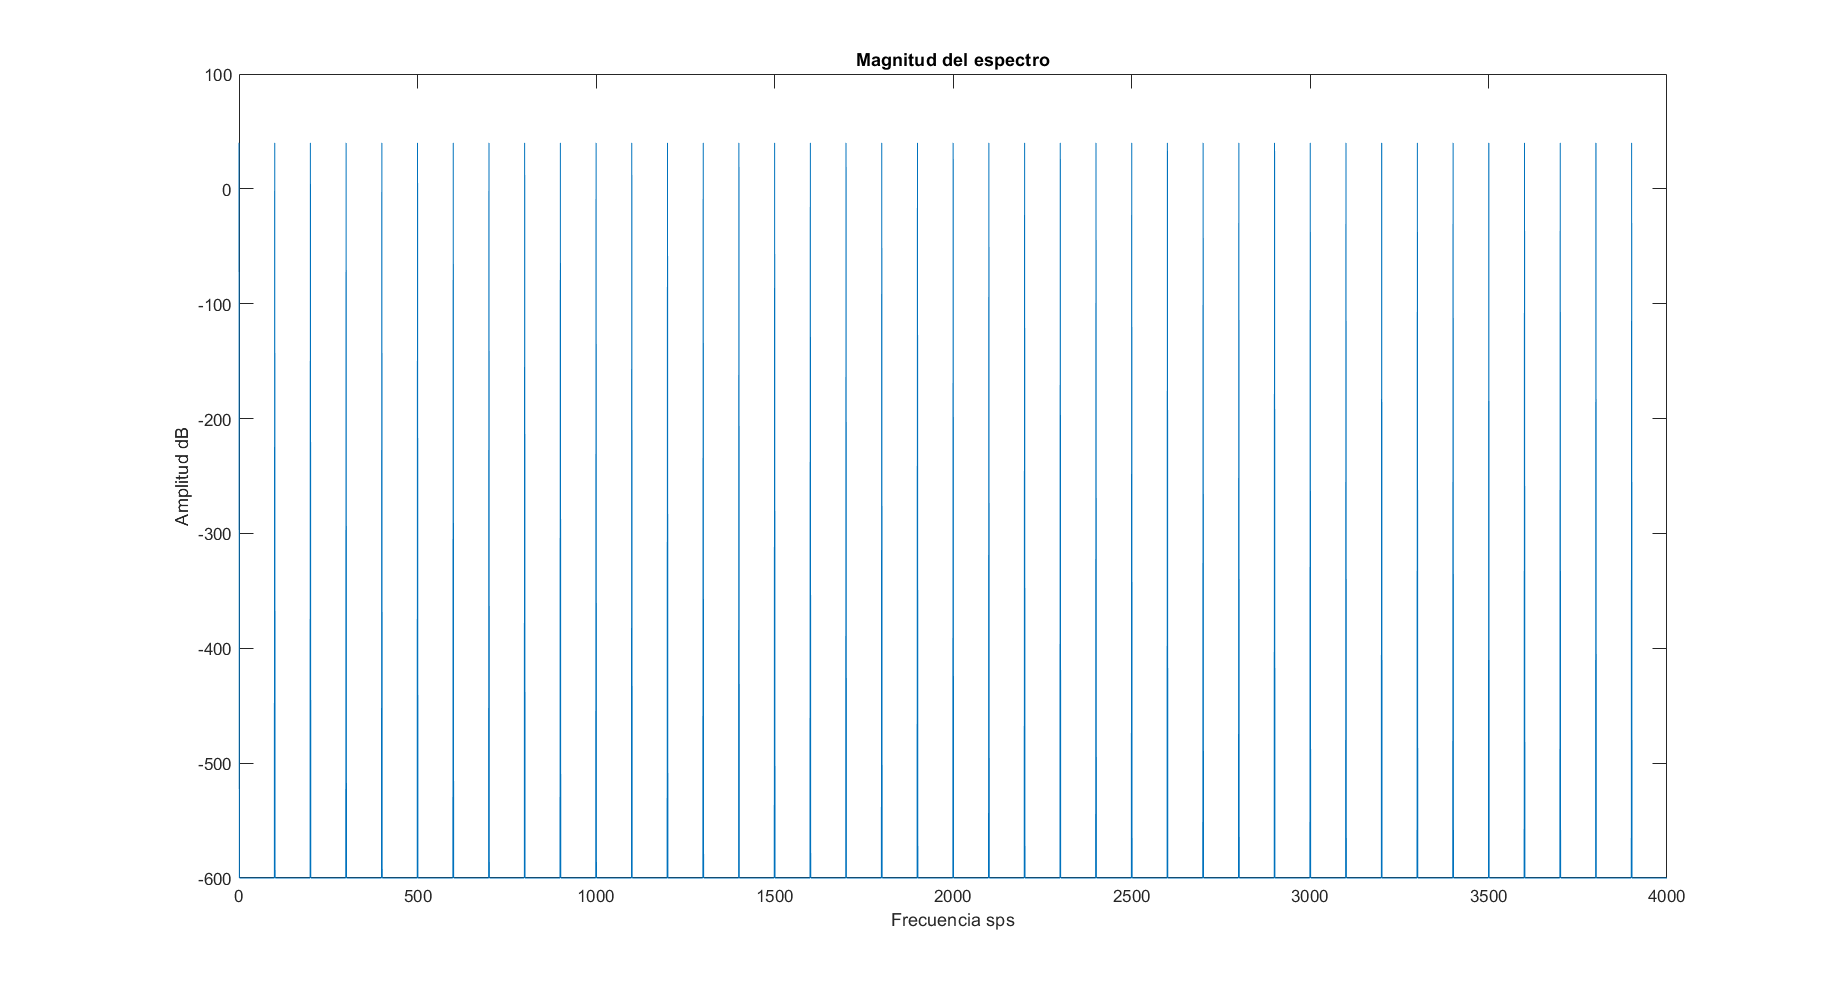
\includegraphics[width=1 \linewidth]{Figuras/P1_1.png}
\caption{Magnitud del espectro de señal generada en dB.}
\label{P1_1}
\end{figure} 
%
%
    \item %2)------------------------------------------------------------------%
%
Se genera cada filtro mediante el comando \textit{lpc} según el siguiente código.
%
\begin{lstlisting}
filtro_x = lpc(vowel_x,15);
X=0;
w = linspace(0,fs,N);
for i=1:1:16
    X=X+filtro_x(i).*exp(-1j*2*pi*w*(i-1));
end
\end{lstlisting}
%
donde $x$ representa la vocal a elección, y $X$ el nombre del filtro para dicha vocal. La magnitud del filtro para cada vocal se muestra en la Figura \ref{P1_2}.

Se observa que cada vocal puede modelarse como un filtro con una respuesta en frecuencia específica.
%
\begin{figure}[H]
\centering
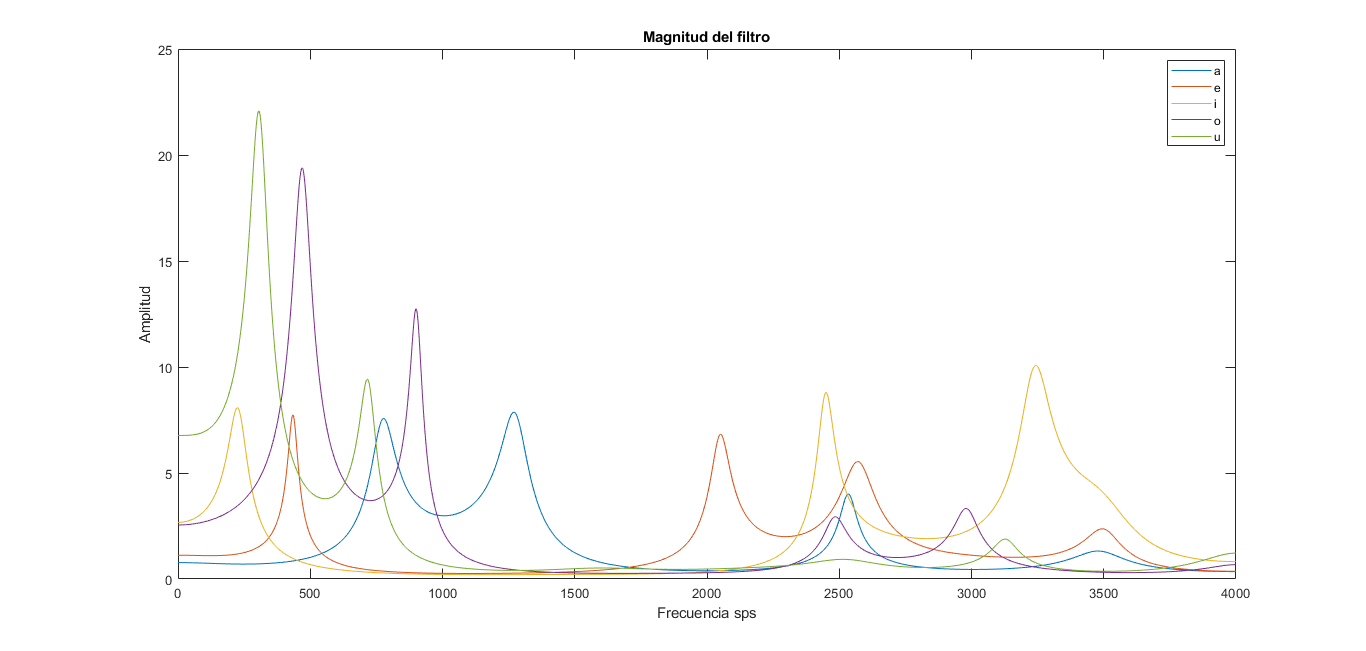
\includegraphics[width=1 \linewidth]{Figuras/P1_2.png}
\caption{Magnitud del espectro del filtro para cada vocal.}
\label{P1_2}
\end{figure} 
%
%Comentarios aqui jaja
%
    \item %3)------------------------------------------------------------------% 
%
    Utilizando los filtros diseñados con el comando \textit{lpc}, se generan vocales sintetizadas filtrando la señal de impulsos generada en 1). 
    
    El código utilizado para aquello es el siguiente:
    \begin{lstlisting}
    fs=8000;
    N=fs;
    Np=80;
    X = exciteV(N,Np);
    v = lpc(vowel_v,15);
    v_sint = filter(1,v,X);
    \end{lstlisting}
    Donde $v = {a,e,i,o,u}$ corresponde a la vocal a sintetizar. $v\_sint$ corresponde a la vocal sintetizada.

    La magnitud en $dB$ del espectro de las señales filtradas se muestra en la figura \ref{P1_3}. Al oír las señales se identifican claramente las vocales, a pesar de que el timbre se la señal no corresponde exactamente al de la voz humana.

%
\begin{figure}[H]
\centering
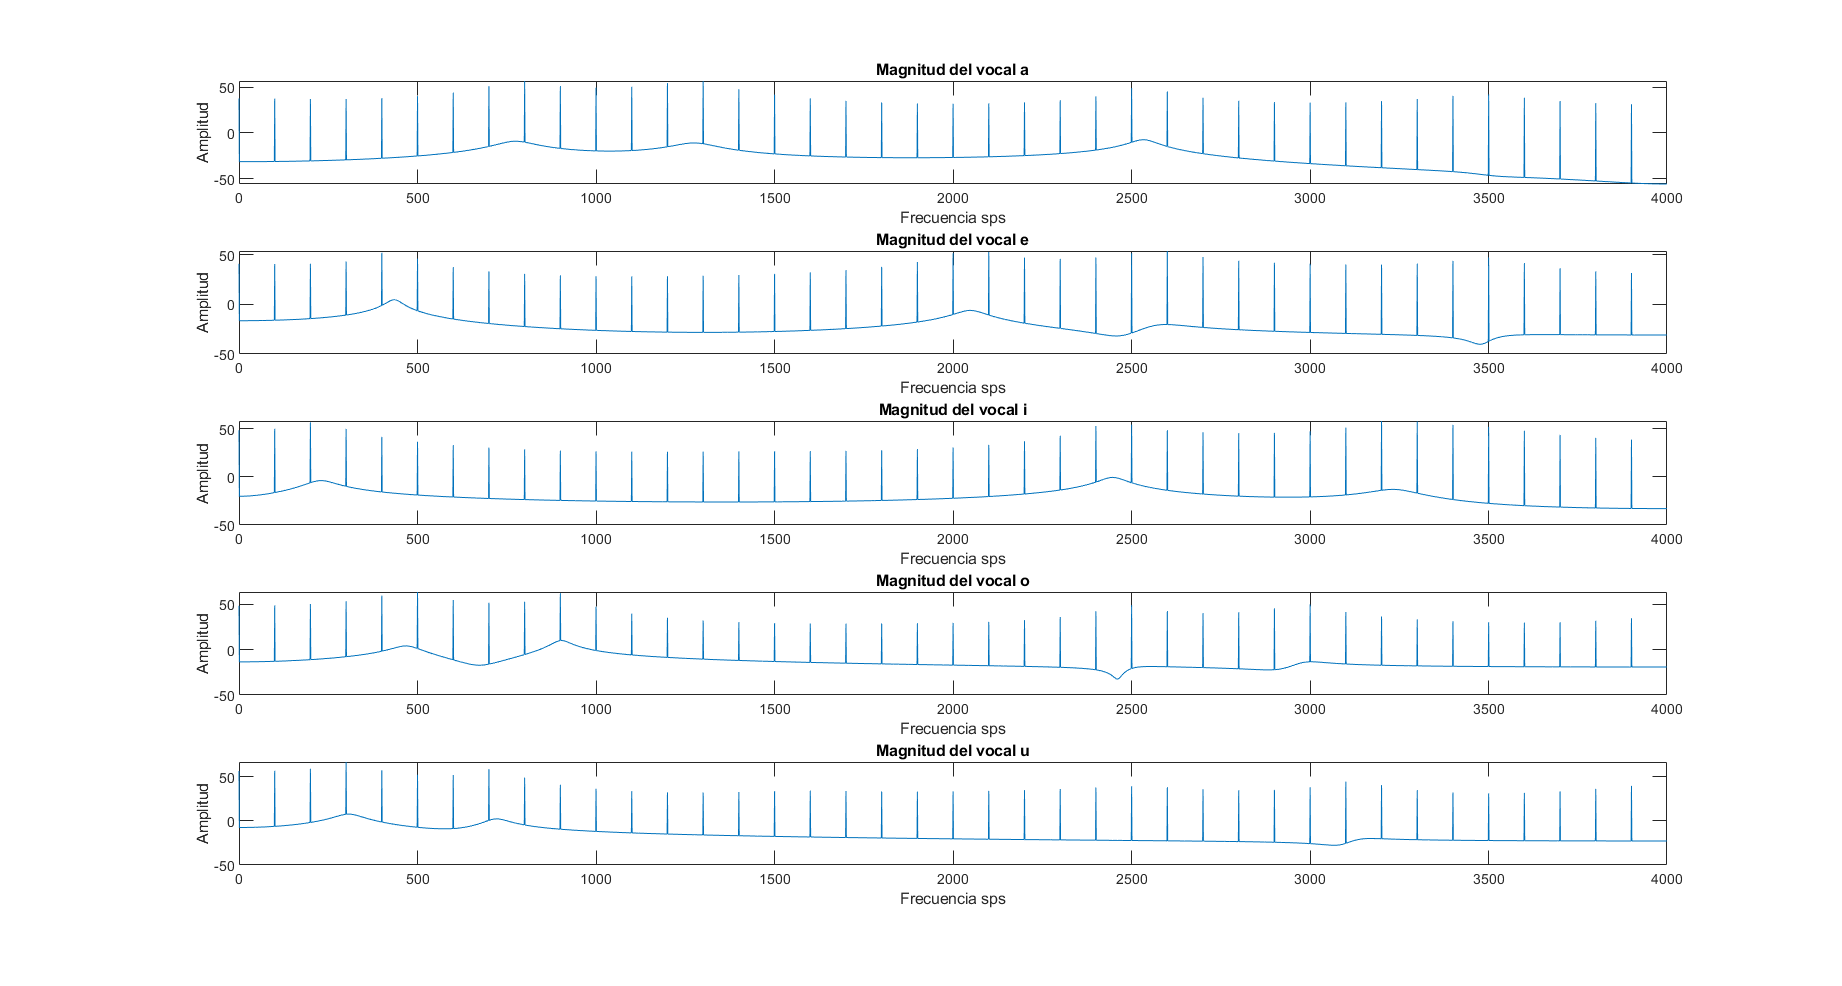
\includegraphics[width=1 \linewidth]{Figuras/P1_3.png}
\caption{Magnitud del espectro de cada vocal en dB.}
\label{P1_3}
\end{figure} 
%
%
    \item %4)------------------------------------------------------------------% 
%
La función $mylpc$ diseñada se muestra a continuación. Cabe notar que se debe agregar el primer coeficiente (que es $1$) a los parámetros obtenidos por la covarianza y la matriz de Toeplitz.

%
\begin{lstlisting}
 function a = mylpc(x,p)
 rx = xcorr(x);
 largo_rx = length(rx);
 rx1 = rx(ceil(0.5*largo_rx)+1:ceil(0.5*largo_rx)+p);
 rx2 = rx(ceil(0.5*largo_rx):ceil(0.5*largo_rx)+p-1);
 Rx = toeplitz(rx2);
 if  det(Rx) == 0
     a = zeros([1,16]);
 else
    a = Rx^(-1)*rx1;
    a = [1; -a];
 end
 end
\end{lstlisting}
%
Los resultados obtenidos se observan en las figuras \ref{P1_4a} y \ref{P1_4b}. Se observa que los filtros y las señales sintetizadas son iguales con el algoritmo de $lpc$ de matlab y el algorítmo $mylpc$ diseñado. Corroborando el funcionamiento correcto de este último.
%
\begin{figure}[H]
\centering
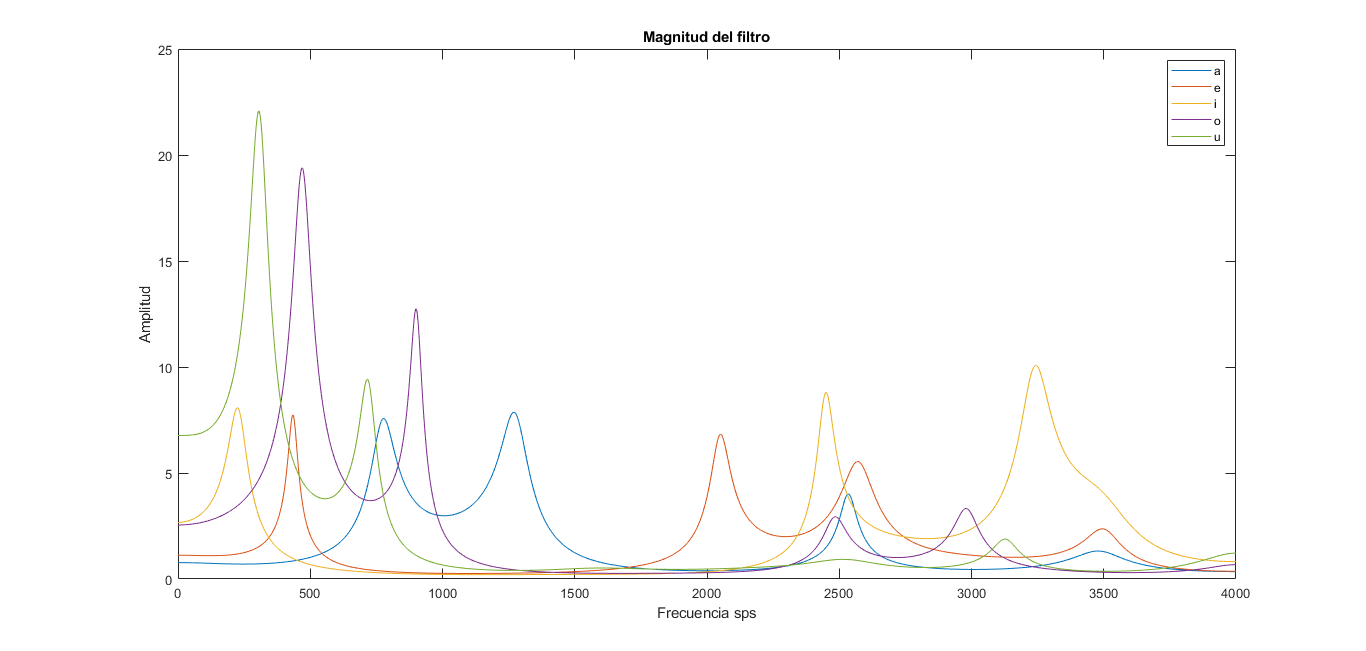
\includegraphics[width=1 \linewidth]{Figuras/P1_4a.png}
\caption{Magnitud del espectro del filtro para cada vocal.}
\label{P1_4a}
\end{figure} 
%
\begin{figure}[H]
\centering
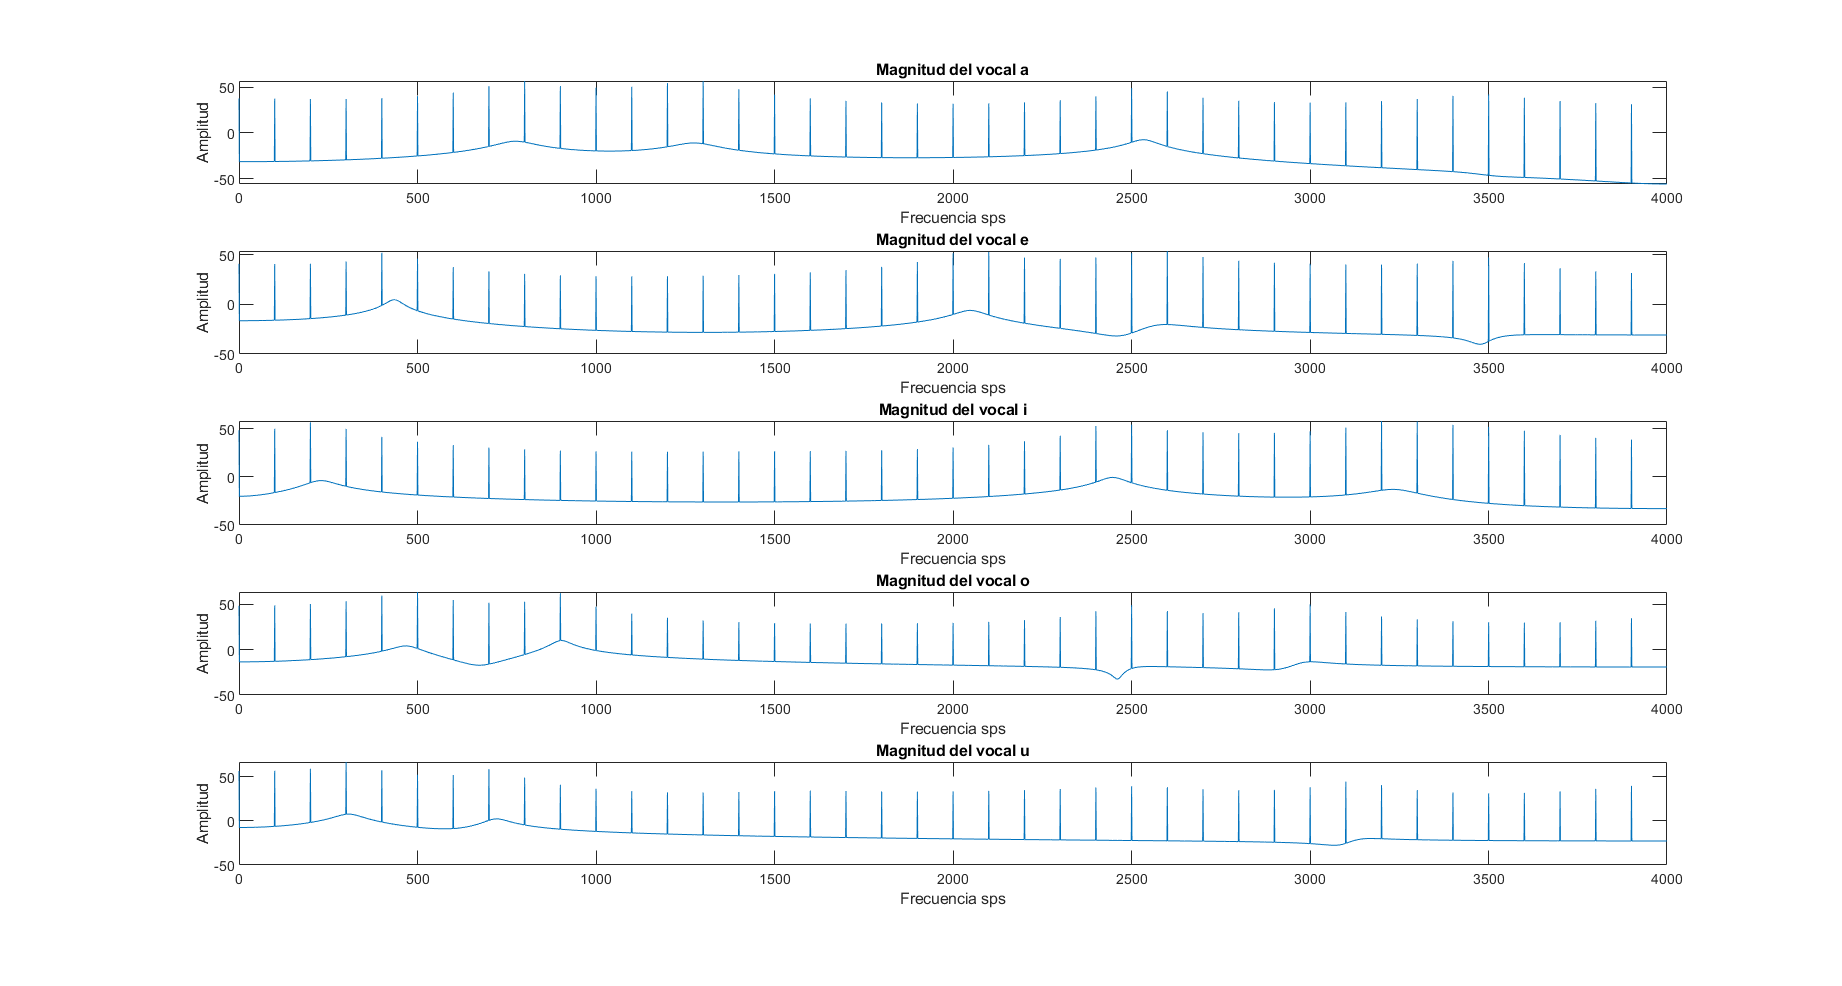
\includegraphics[width=1 \linewidth]{Figuras/P1_4b.png}
\caption{Magnitud del espectro de cada vocal en dB.}
\label{P1_4b}
\end{figure} 
%
\end{enumerate}
%%%%%%%%%%%%%%%%%%%%%%%%%%%%%%%%%%%%%%%%%%%%%%%%%%%%%%%%%%%%%%%%%%%%%%%%%%%%%%%%%
%
%-------------II. Clasificación de segmentos VUS----------------------------%
%
%%%%%%%%%%%%%%%%%%%%%%%%%%%%%%%%%%%%%%%%%%%%%%%%%%%%%%%%%%%%%%%%%%%%%%%%%%%%%%%%%
\section{Clasificación de segmentos VUS}
\begin{enumerate}[1)]
    \item %1)------------------------------------------------------------------%
Se carga la señal \textit{training\_signal} para realizar el entrenamiento de clasificación de segmentos VUS.    

En primer lugar, se utiliza el comando \textit{ginput} para seleccionar la señal en distintos fragmentos correspondientes a vocales, consonantes y silencio. El gráfico obtenido según aquello se muestra en la figura\ref{P2}.
\begin{figure}[H]
    \centering
    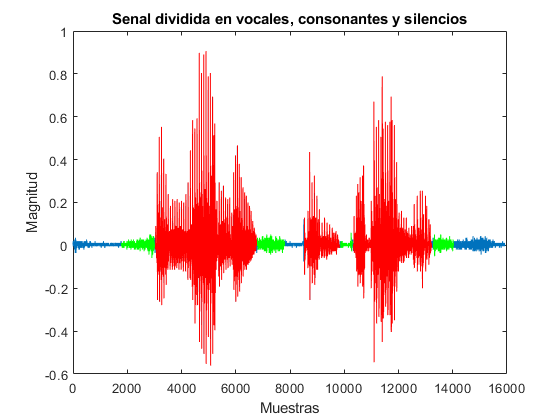
\includegraphics[width = 0.9 \linewidth]{Figuras/P2.png}
    \caption{Señal dividida en silencio (azul), consonantes (verde) y vocales (rojo)}
    \label{P2}
\end{figure}

Para un análisis mas riguroso, se decide separar la señal en cada letra, calculando para cada una el valor RMS, y si cantidad de cruces por cero por segundo, la cual está dada por la siguiente función.

\begin{lstlisting}
 function y = cruces_cero(x)
 largo_senal = length(x)/8000*1000;
 y=0;
  for i=2:length(x)
    if (x(i)*x(i-1))<0
      y=y+1;
    end
  end
  y=y/largo_senal;
 end
\end{lstlisting}

Se separan las letras en vocales, y se utiliza un \textit{scatter plot} para obtener sus valores RMS vs sus cruces por cero por segundo. La gráfica obtenida se muestra en la figura \ref{P2_1}.

Se observa que el valor RMS parecería ser un mejor criterio que la cantidad de cruces por cero para identificar si una señal es vocal, consonante o silencio. Sin embargo resulta más conveniente utilizar una combinación de ambos criterios para decidir si la señal es vocal o consonante.
%
\begin{figure}[H]
\centering
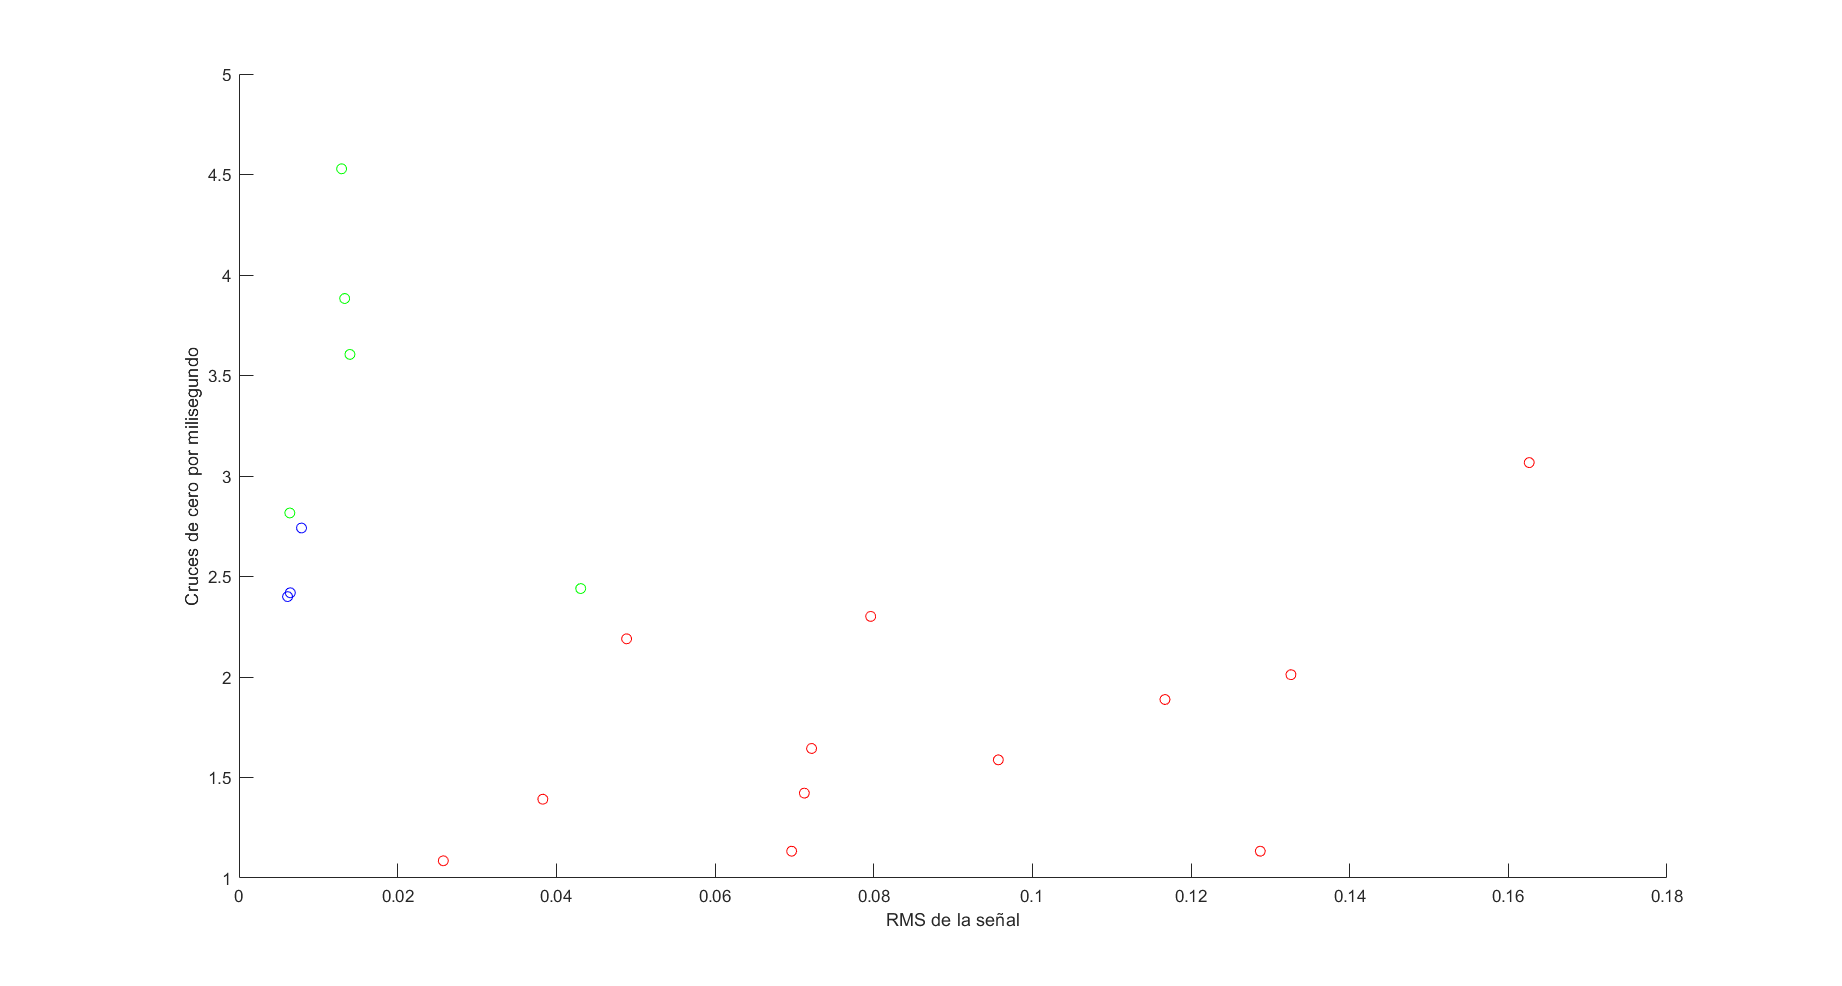
\includegraphics[width=1 \linewidth]{Figuras/P2_1.png}
\caption{RMS y cruces de la señal.}
\label{P2_1}
\end{figure} 
%
    \item %2)------------------------------------------------------------------% 
    A partir de los resultados del gráfico del punto anterior, se utiliza el criterio descrito en la siguiente función para clasificar si la señal es vocal, consonante o silencio. Donde $y=0$ representa los frames donde hay silencio, $y=-1$ representa los frames donde hay una consonante y $y=1$ representa los frames donde hay una vocal.
    \begin{lstlisting}
    function y = find_VUS(x)
    if(rms(x)<0.02)
        y = 0;
    else
        if(cruces_cero(x)>2.4 && rms(x)<0.06)
            y = -1;
        else
            y = 1;
        end
    end
    end
    \end{lstlisting}
    Se calcula el valor VUS de cada frame de la señal de prueba y se almacena en un vector. Se grafica la señal junto a la variable VUS en la figura \ref{P2_2}. 
    
    A simple vista los valores obtenidos parecen ser consistentes con los sonidos vocales (secciones donde se identifica una señal períodica), consonantes (secciones más similares a ruido blanco) y silencios (secciones donde no hay nada) en la señal.
    \begin{figure}[H]
        \centering
        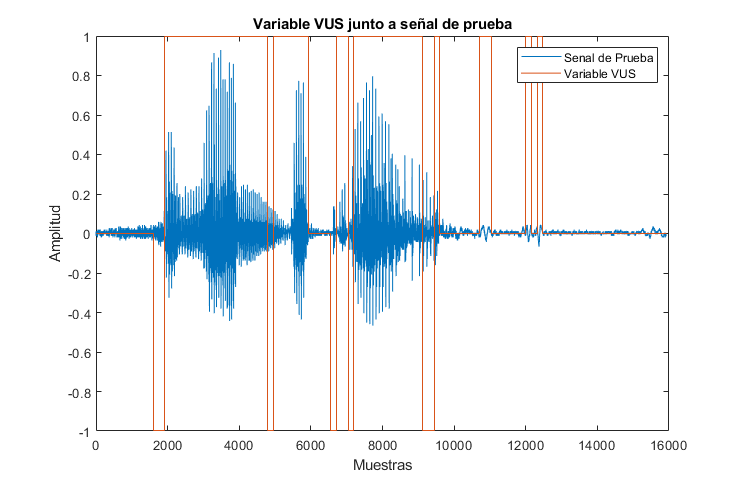
\includegraphics[width=0.9 \linewidth]{Figuras/P2_2.png}
        \caption{Valor VUS obtenido para cada frame de la señal}
        \label{P2_2}
    \end{figure}
\end{enumerate}
%%%%%%%%%%%%%%%%%%%%%%%%%%%%%%%%%%%%%%%%%%%%%%%%%%%%%%%%%%%%%%%%%%%%%%%%%%%%%%%%%
%
%---------III. Sintesis de voz hablada-------------------%
%
%%%%%%%%%%%%%%%%%%%%%%%%%%%%%%%%%%%%%%%%%%%%%%%%%%%%%%%%%%%%%%%%%%%%%%%%%%%%%%%%%
\section{Síntesis de voz hablada}
\begin{enumerate}[1)]
    \item %1)------------------------------------------------------------------%
A partir de la señal a comprimir se genera un vector con los coeficientes VUS de cada frame, un vector con el valor RMS de cada frame y una matriz con los coeficientes LPC de cada frame
\begin{lstlisting}
for i=1:100
    i2 = 0.02*fs*(i-1)+1;
    frame = test_signal(i2:i2+min(0.02*fs-1,length(test_signal)-i2));
    VUS_vector(i)=find_VUS(frame);
    RMS_vector(i)=rms(frame);
    lpc_matrix(:,i) = mylpc(frame,15);
end
\end{lstlisting}
Esos valores son los datos que el emisor debe enviar al receptor en lugar de la señal completa. \\

Luego, se genera la señal sintetizada a partir de los vectores (que en caso de comunicación real son los datos que debieron haber llegado al receptor). Donde la señal a filtrar depende del flag VUS correspondiente a cada frame.

\begin{lstlisting}
senal_sintetizada = zeros([1,length(test_signal)]);
for j=1:100
    j2 = 0.02*fs*(j-1)+1;
    if VUS_vector(j)==0
        senal_sintetizada(j2:j2+min(0.02*fs-1,length(test_signal)-j2-1)) =
                    zeros(1,min(0.02*fs,length(test_signal)-j2));
    else
        if VUS_vector(j)==1
            X = exciteV(min(0.02*fs,length(test_signal)-j2),80);
            rmsfactor = RMS_vector(i)/rms(filter(1,lpc_matrix(:,j),X));
            senal_sintetizada(j2:j2+min(0.02*fs-1,length(test_signal)-j2-1)) =
                        filter(1,lpc_matrix(:,j),X)*rmsfactor;
        else
            X = rand([1,min(0.02*fs,length(test_signal)-j2)]);
            rmsfactor = RMS_vector(i)/rms(filter(1,lpc_matrix(:,j),X));
            senal_sintetizada(j2:j2+min(0.02*fs-1,length(test_signal)-j2-1)) =
                        filter(1,lpc_matrix(:,j),X)*rmsfactor;
        end
    end
end
\end{lstlisting}

La señal sintetizada obtenida junto a la señal original se muestran en la Figura \ref{P3_1}.

Al escuchar la señal creada, se identifica correctamente la frase del audio original, y el tono es relativamente similar a la voz humana, aunque sigue siendo apreciable que es una señal generada por computador. \\

Para mejorar la síntesis, se podrían considerar los cambios de frecuencia que tiene la voz humana al hablar, agregar mayor orden al filtro (aunque eso implica enviar más datos por el canal), además de quizás cambiar la  señal de base para el filtrado al residuo calculado con el filtro inverso de voces reales.
%
\begin{figure}[H]
    \centering
    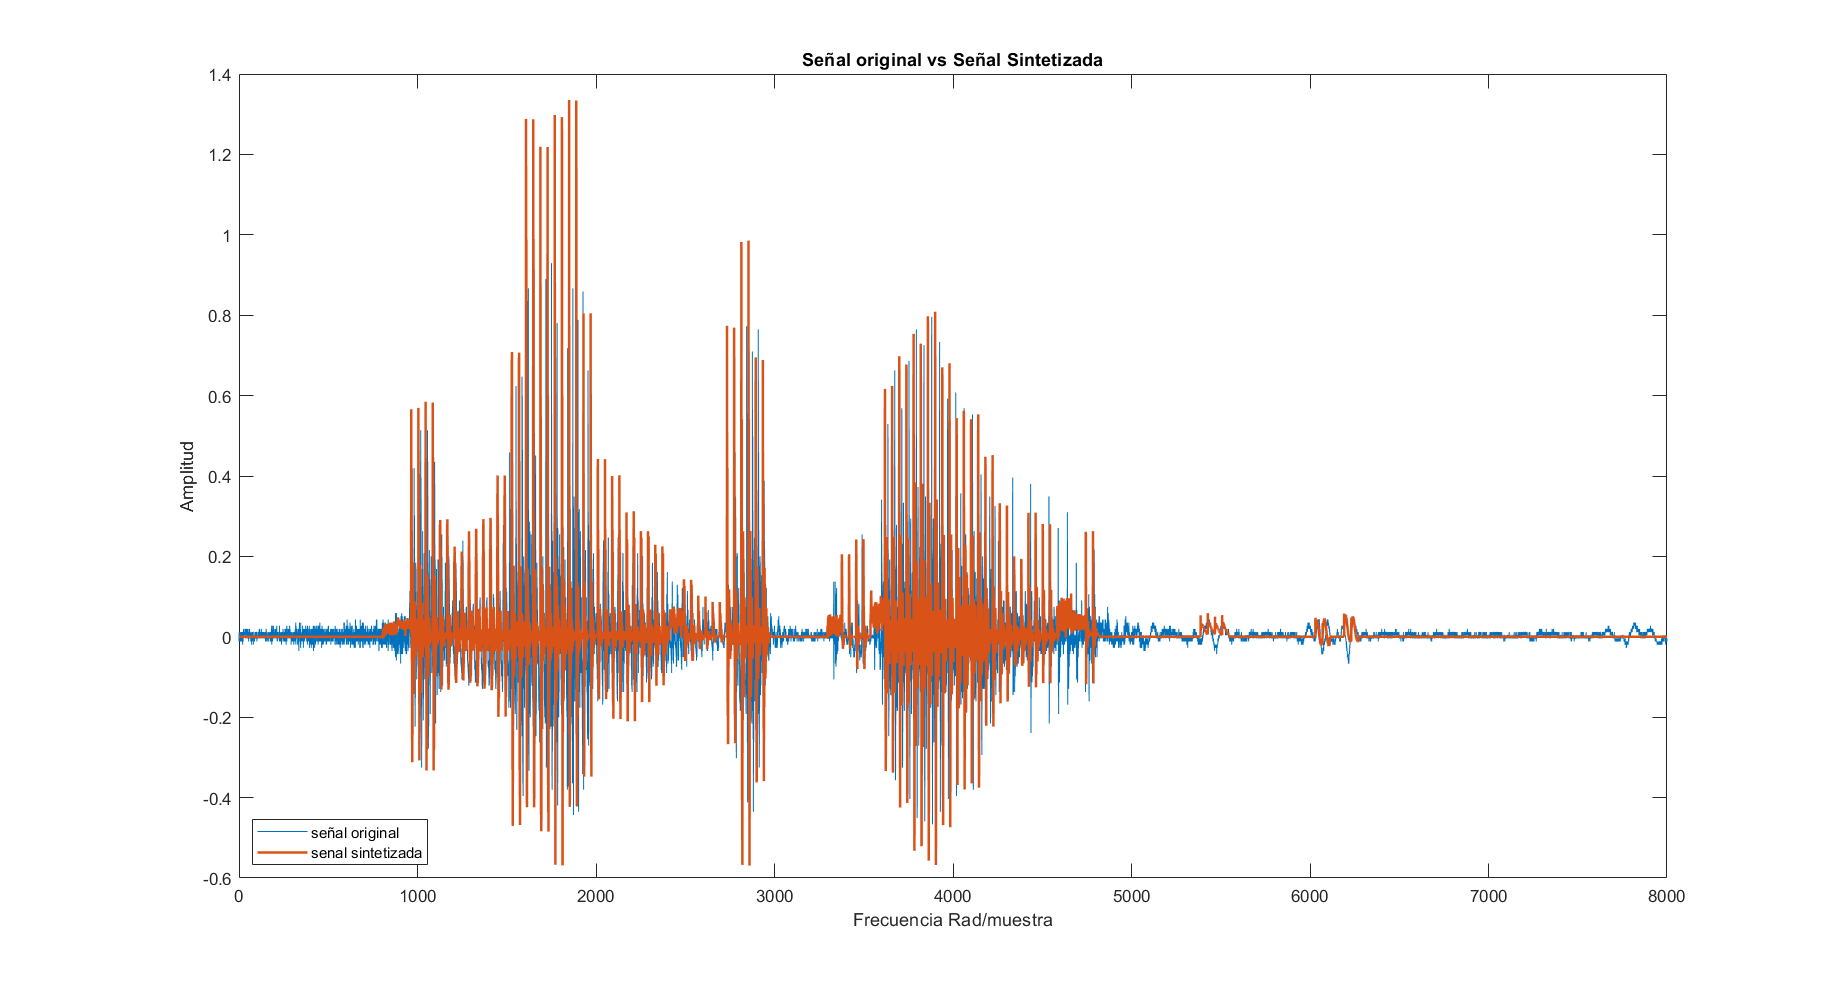
\includegraphics[width = 0.9 \linewidth]{Figuras/P3_1.png}
    \caption{Señal de prueba vs señal sintetizada.}
    \label{P3_1}
\end{figure}
%
    \item %2)------------------------------------------------------------------% 
%
La cantidad de bytes necesarios para almacenar la señal original es de $127360$.

La cantidad de bytes necesarios para almacenar el vector de flags VUS es $800$, la cantidad para el vector de valores RMS es $800$ y la cantidad para la matriz de coeficientes lpc es $12800$. Por lo tanto los bytes necesarios para almacenar la señal comprimida son $14400$.

Por lo tanto la razón de compresión es de $8.84$.

%
\end{enumerate}
%%%%%%%%%%%%%%%%%%%%%%%%%%%%%%%%%%%%%%%%%%%%%%%%%%%%%%%%%%%%%%%%%%%%%%%%%%%%%%%%%
%
%---------FILTRO AUTOREGRESIVO-----------------%
%
%%%%%%%%%%%%%%%%%%%%%%%%%%%%%%%%%%%%%%%%%%%%%%%%%%%%%%%%%%%%%%%%%%%%%%%%%%%%%%%%%
\section{Filtro Autoregrecivo}
\begin{enumerate}[1)]
\item %1)------------------------------------------------------------------% 
%
La función $positiveSpectrum$ se muestra a continuación.
%
\begin{lstlisting}
function Y = positiveSpectrum(X)
Spectrum = abs(fft(X));
Y = Spectrum(1:floor(length(X)/2)+1);
end

function X = exciteV (N, Np)
  for i=1:1:N
    if mod(i-1,Np) == 0
      X(i)=1;
    else
      X(i)=0;
    end
  end
 end
\end{lstlisting}
%
El espectro de la señal $Vowel\_a$ se muestra en la Figura \ref{P4_1}, donde se reconocen aproximadamente $5$ formantes.
% cuantos formantes se reconocen
%
\begin{figure}[H]
    \centering
    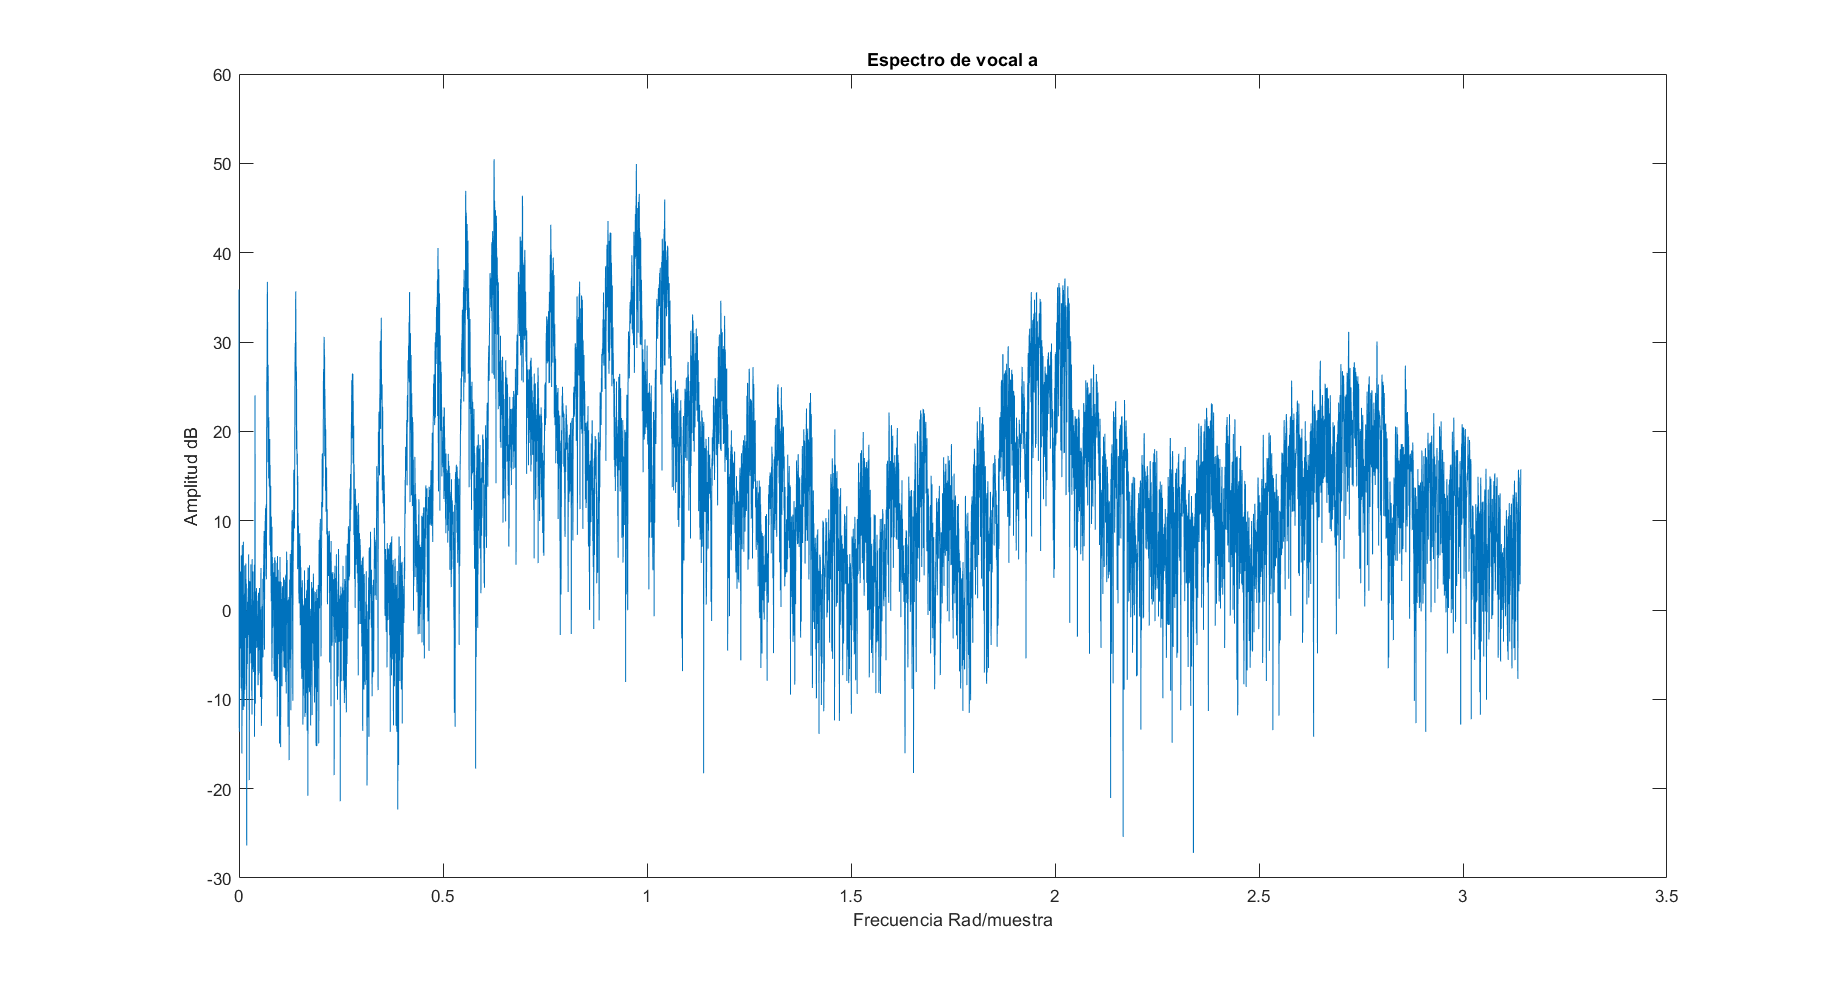
\includegraphics[width = 0.9 \linewidth]{Figuras/P4_1.png}
    \caption{Espectro de la Vocal A.}
    \label{P4_1}
\end{figure}
%
\item %2)------------------------------------------------------------------%
Se probarón filtros lpc de orden $2$ y $15$ para las vocales $a$ y $u$.

Los filtros probados se muestran junto al espectro de las señales en las Figuras \ref{P4_2A} y \ref{P4_2U}.
%
\begin{figure}[H]
    \centering
    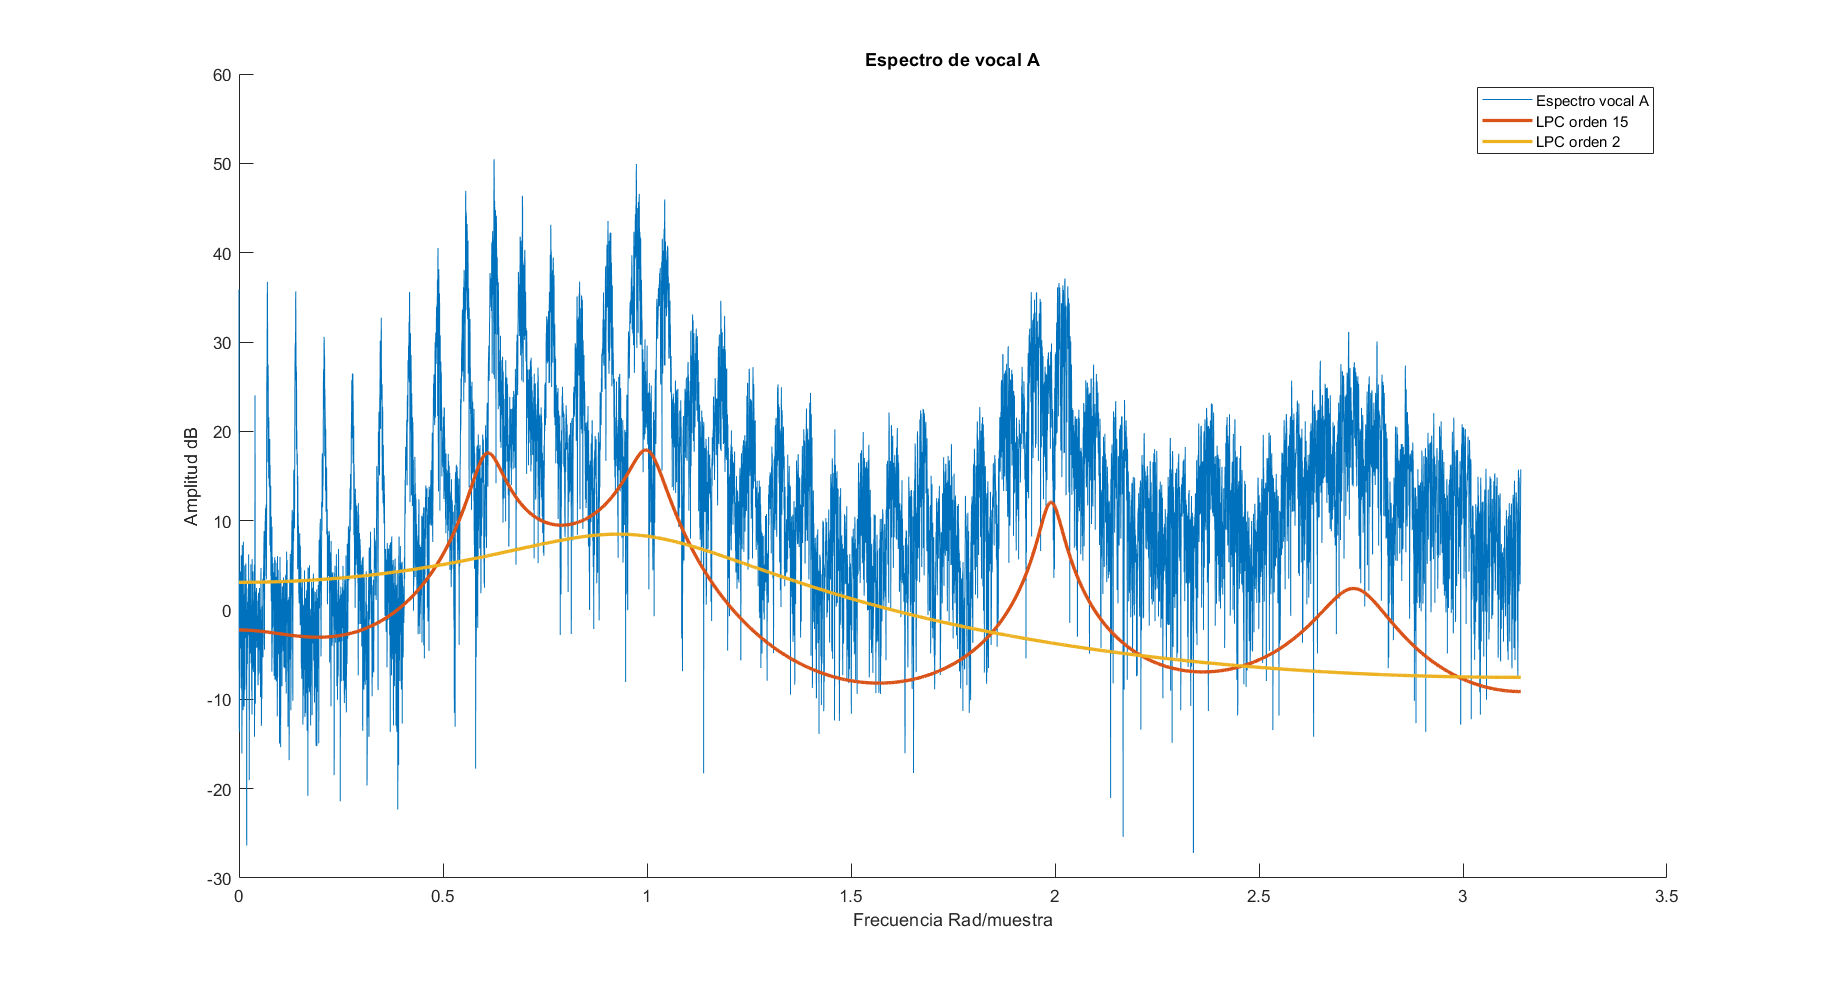
\includegraphics[width = 0.9 \linewidth]{Figuras/P4_2A.png}
    \caption{Espectro y LPC de vocal A.}
    \label{P4_2A}
\end{figure}
%
\begin{figure}[H]
    \centering
    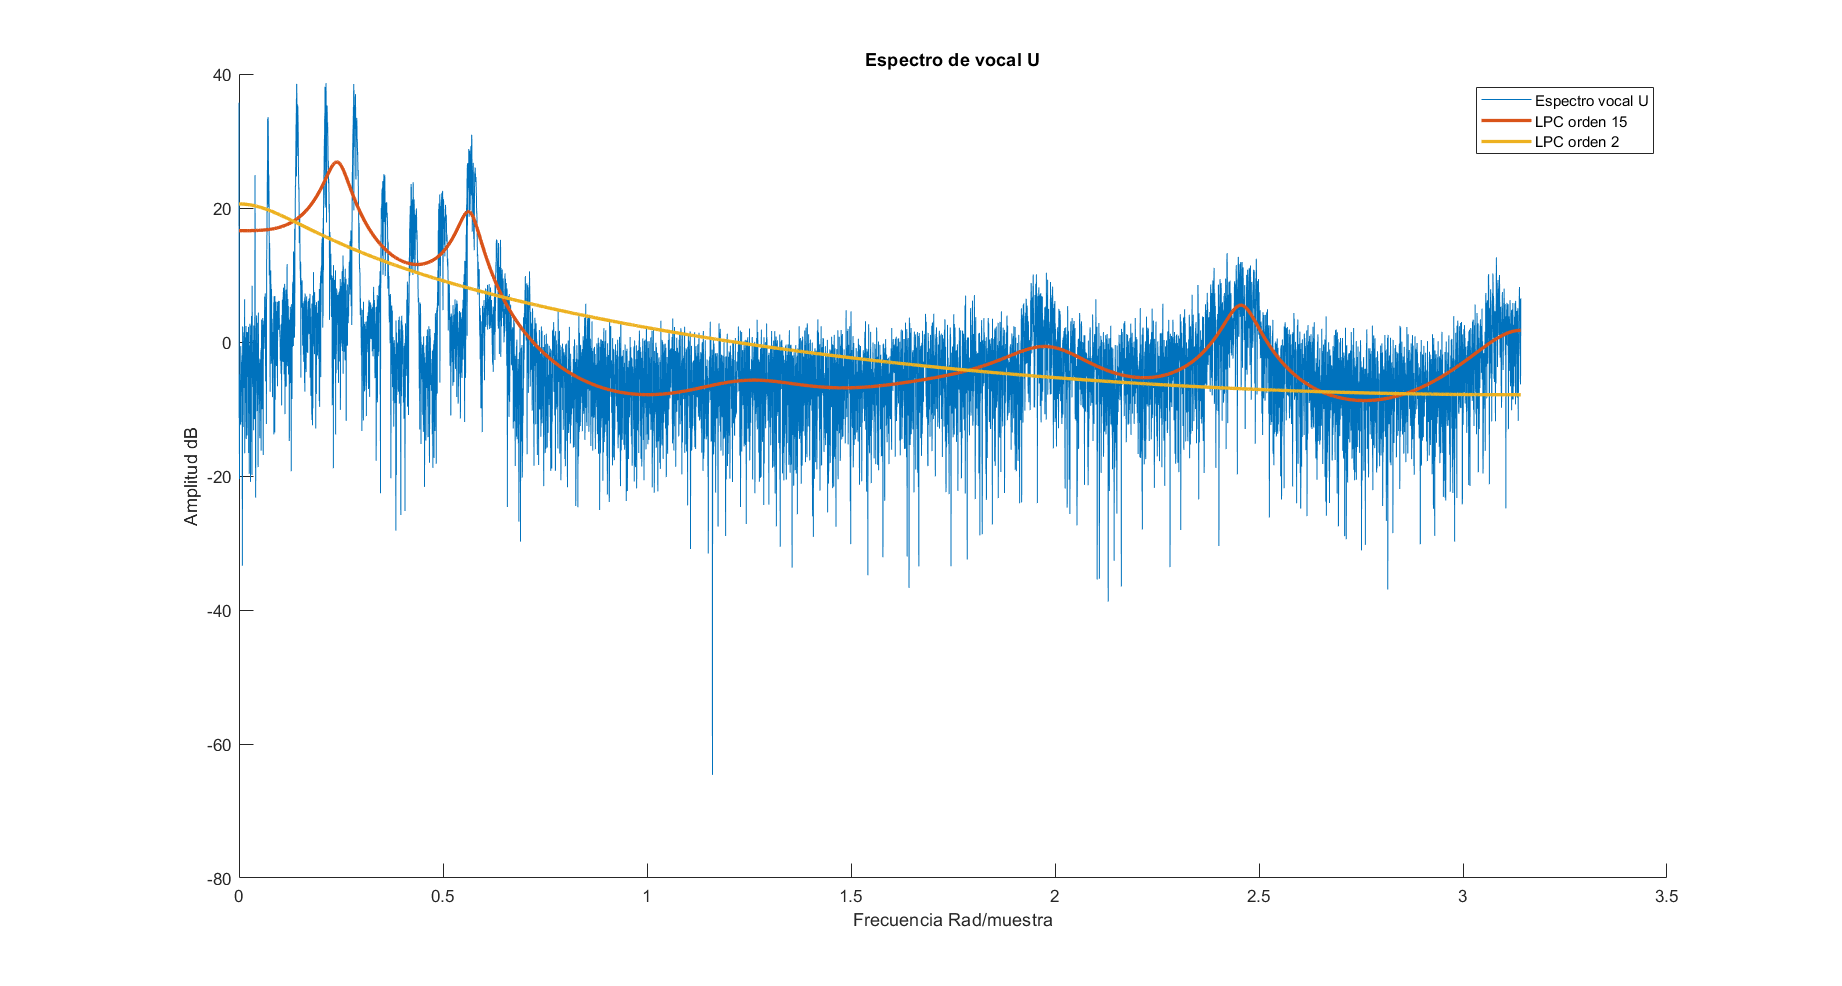
\includegraphics[width = 0.9 \linewidth]{Figuras/P4_2U.png}
    \caption{Espectro y LPC de vocal U.}
    \label{P4_2U}
\end{figure}
%

En la Figura \ref{P4_2Z} se muestra el plano Z para los filtros de distintos ordenes.
%
\begin{figure}[H]
    \centering
    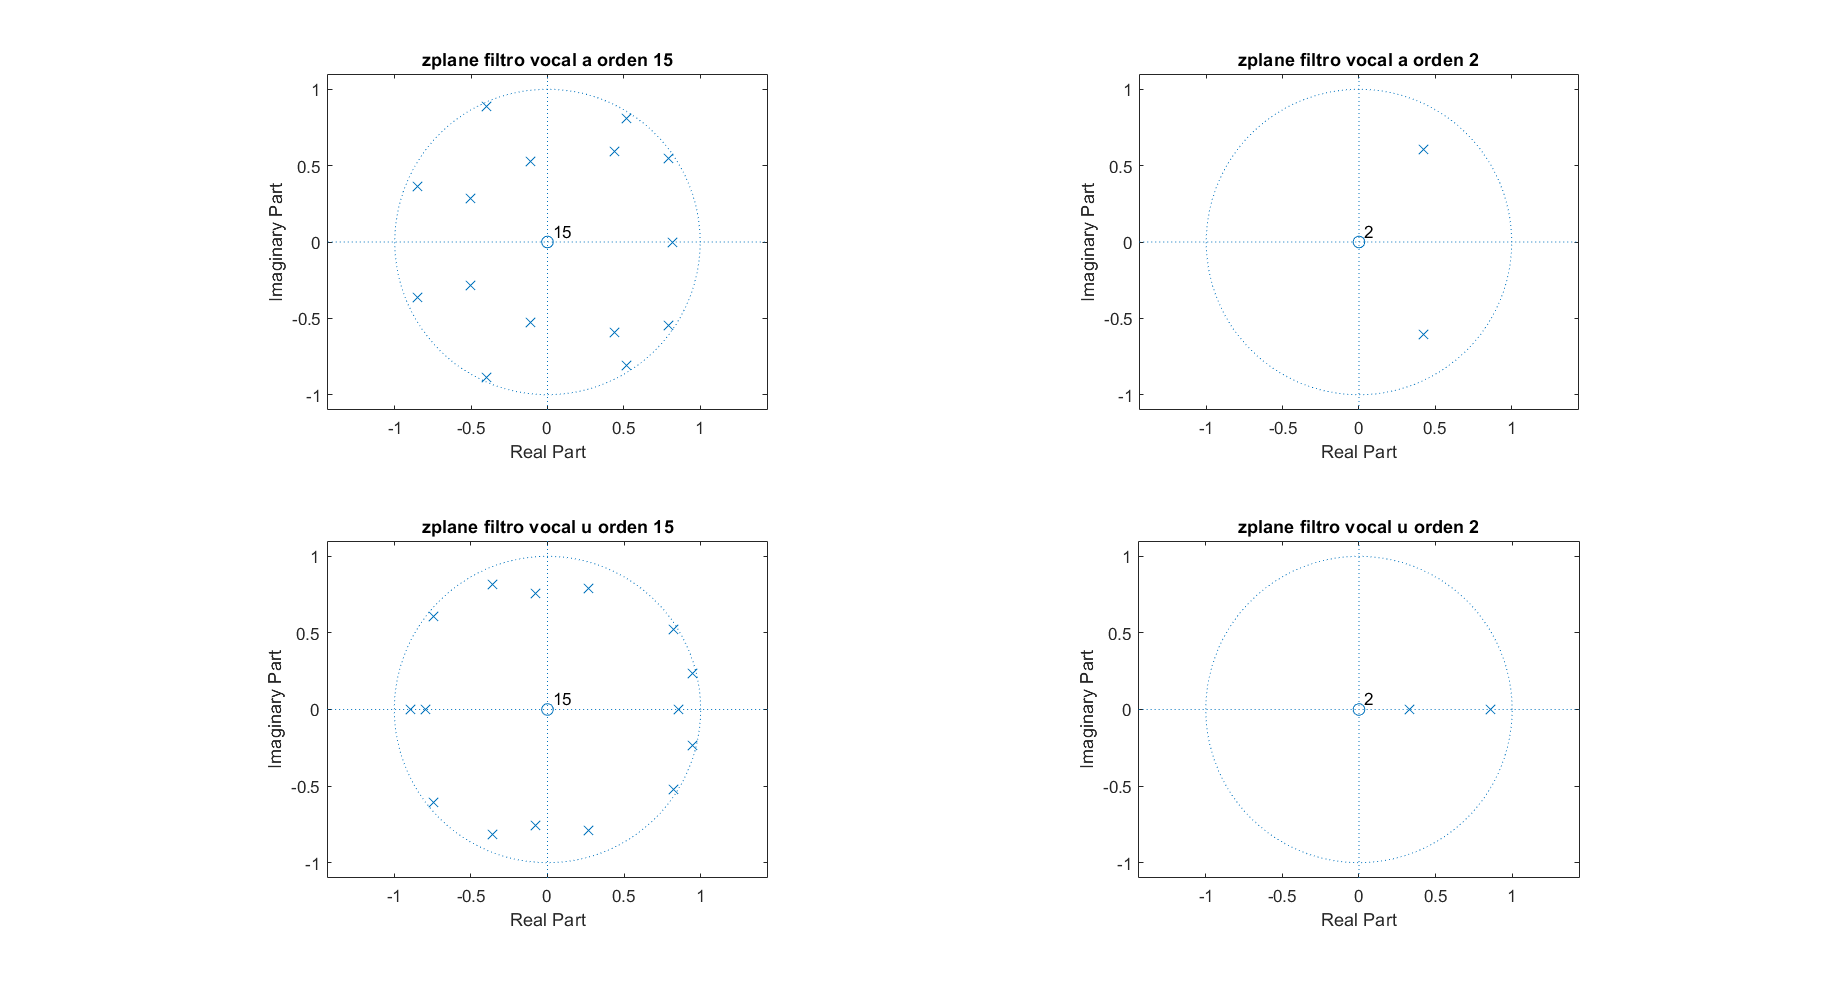
\includegraphics[width = 0.9 \linewidth]{Figuras/P4_2Z.png}
    \caption{Planos Z de vocales A y U para distintos ordenes.}
    \label{P4_2Z}
\end{figure}

La respuesta en frecuencia obtenida por el algoritmo \textit{lpc} de orden $2$ no alcanza a imitar el comportamiento de las vocales, ya que estas tienen una cantidad de formantes mayores a aquel orden. 
Se observa que en el caso de la vocal \textit{a}, los polos de esta aproximación son complejos conjugados, mientras que para la vocal \textit{u} son dos polos reales. \\

\item %3)------------------------------------------------------------------% 
La comparación de los espectros de la vocal \textit{a} original y sintetizada con ordenes $9$ y $15$ se muestra en la Figura \ref{P4_3M_a}. El plano Z para dichos filtros en la Figura \ref{P4_3Z_a}.

No se aprecian diferencias significativas en ambos casos ya que el orden $9$ es suficiente para la cantidad de formantes del espectro de la vocal \textit{a}.

%
\begin{figure}[H]
    \centering
    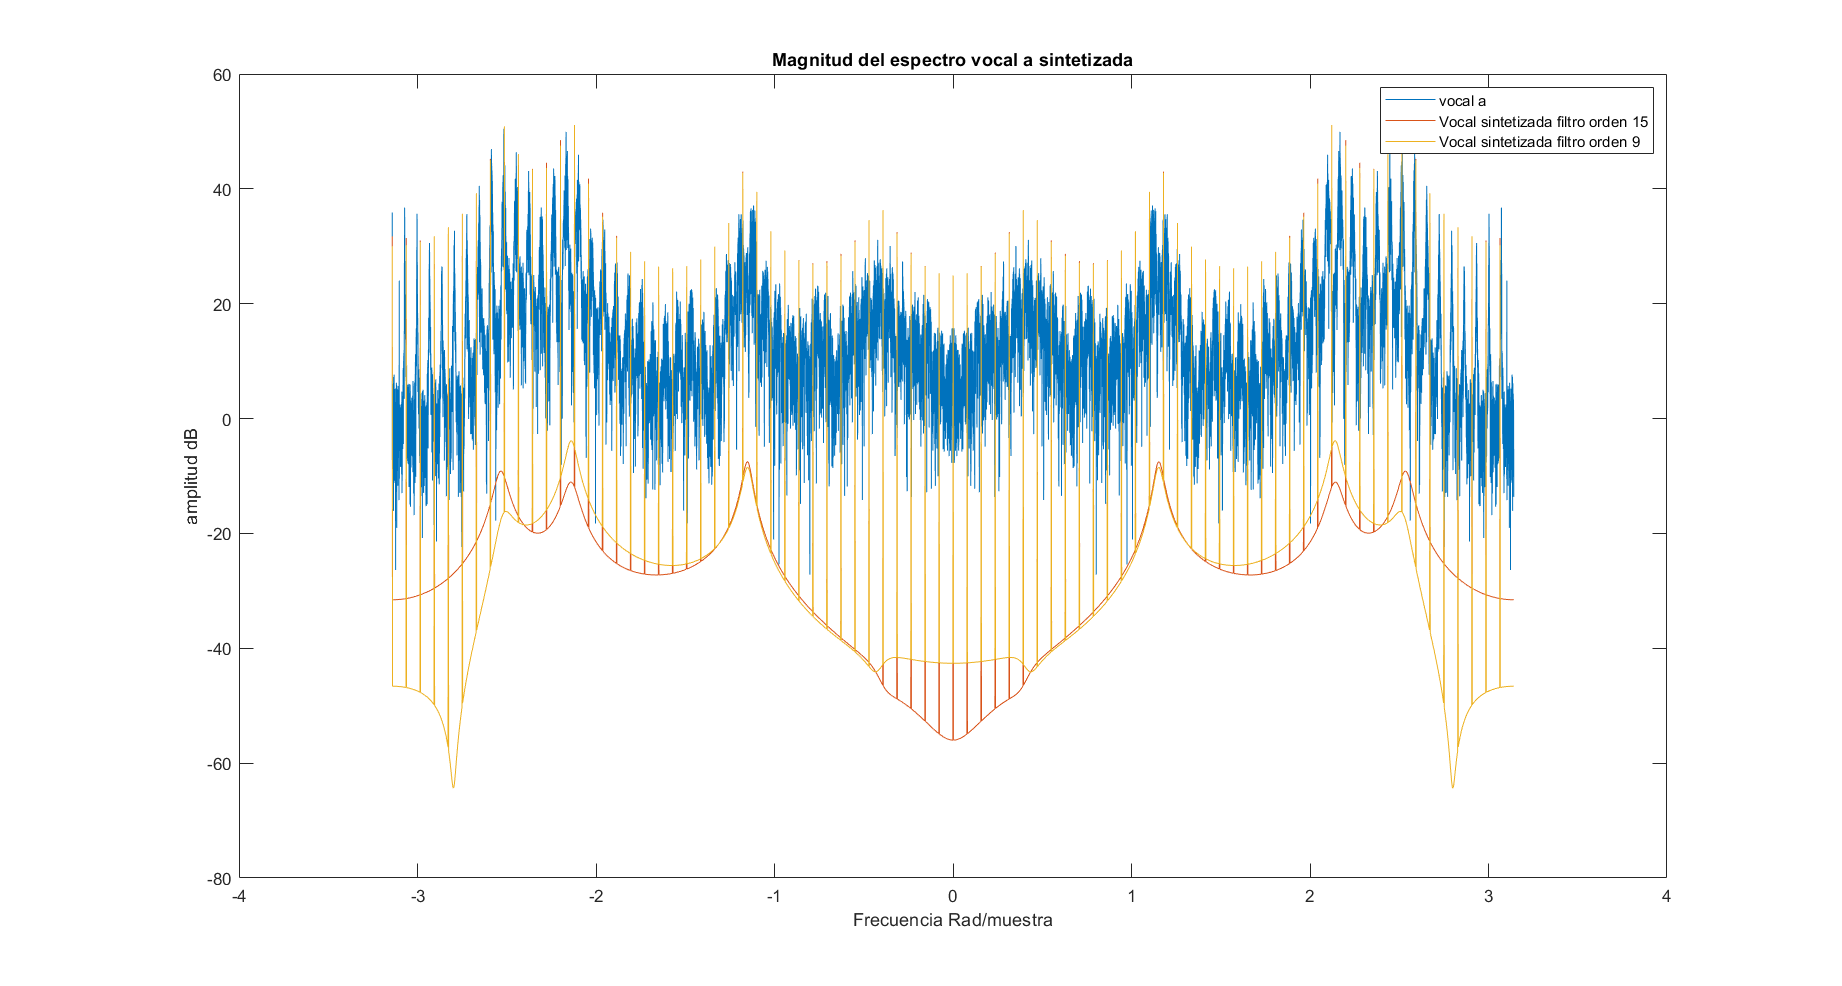
\includegraphics[width = 0.9 \linewidth]{Figuras/P4_3M_a.png}
    \caption{Magnitud de la vocal 'a' origínenla y sintetizada.}
    \label{P4_3M_a}
\end{figure}
%
\begin{figure}[H]
    \centering
    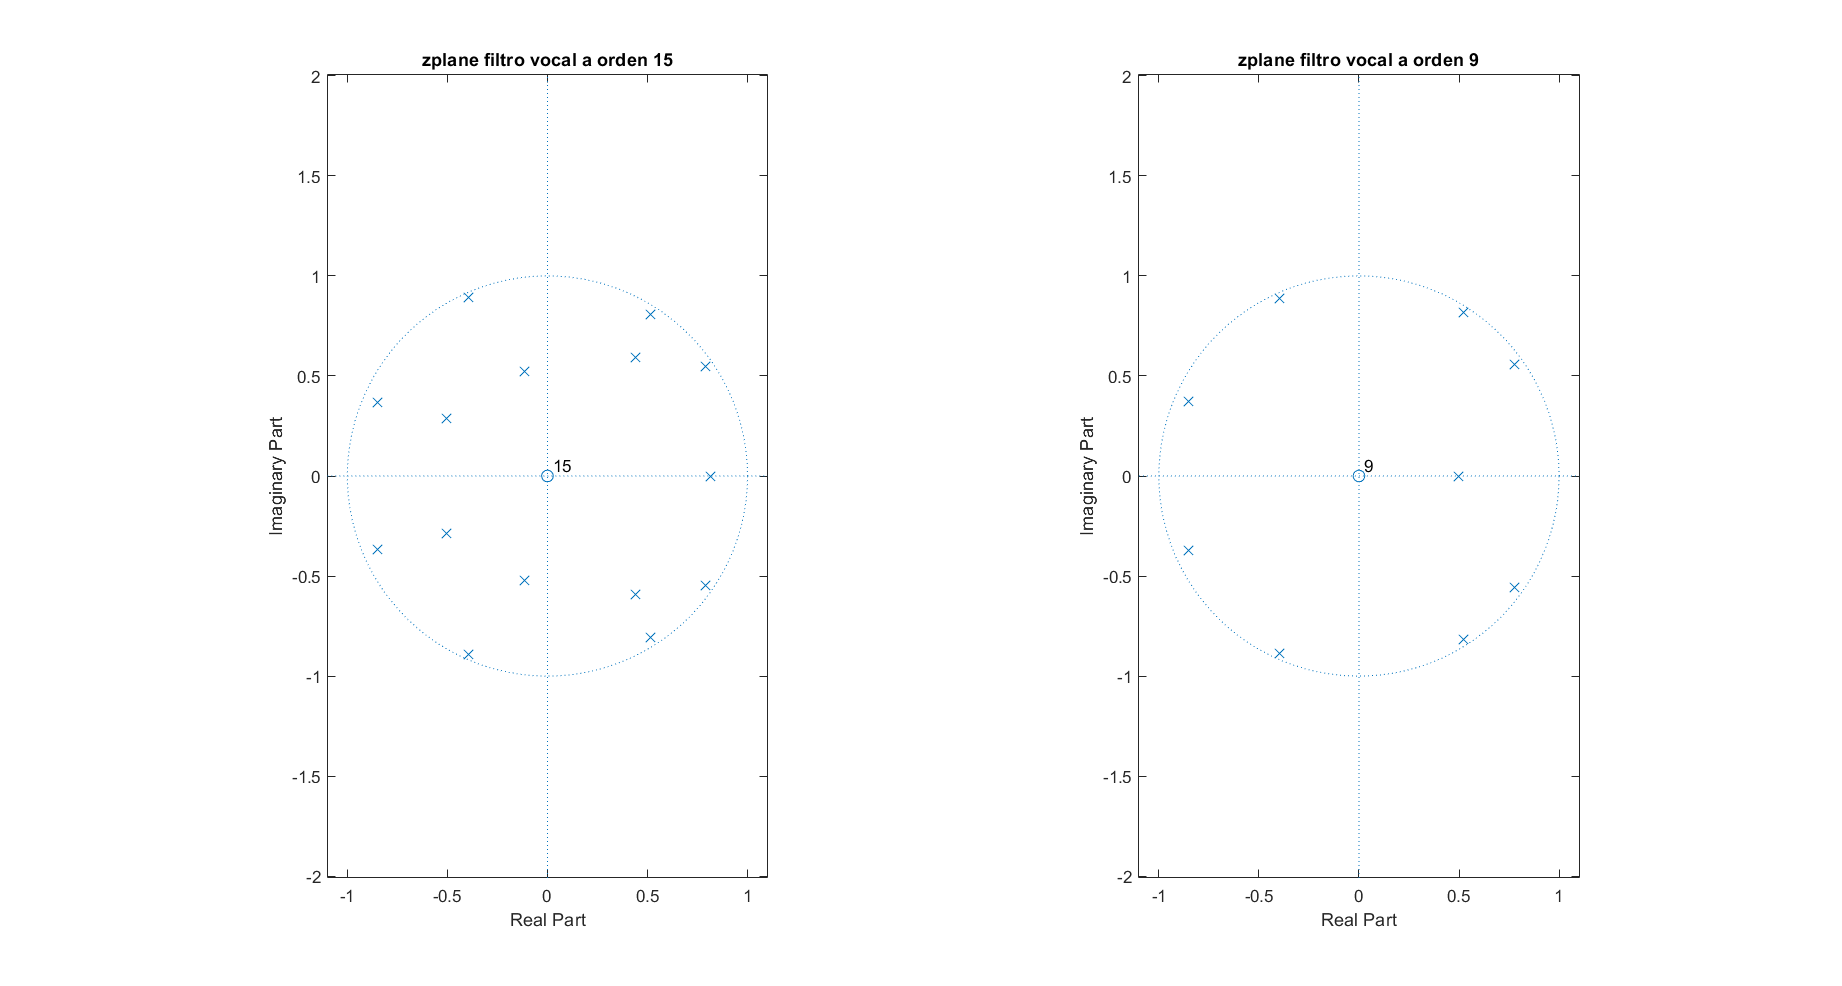
\includegraphics[width = 0.9 \linewidth]{Figuras/P4_3Z_a.png}
    \caption{Planos Z de vocal 'a' para distintos ordenes de filtro.}
    \label{P4_3Z_a}
\end{figure}
%
Para la vocal \textit{u}, el mínimo orden del filtro para el cual no se aprecia diferencia respecto al filtro de orden $15$, es $12$.

La comparación de los espectros de la vocal original, y la vocal sintetizada con ambos ordenes se muestran en la Figura \ref{P4_3M_u}, y el plano Z para dichos filtros en la Figura \ref{P4_3Z_u}.
%
\begin{figure}[H]
    \centering
    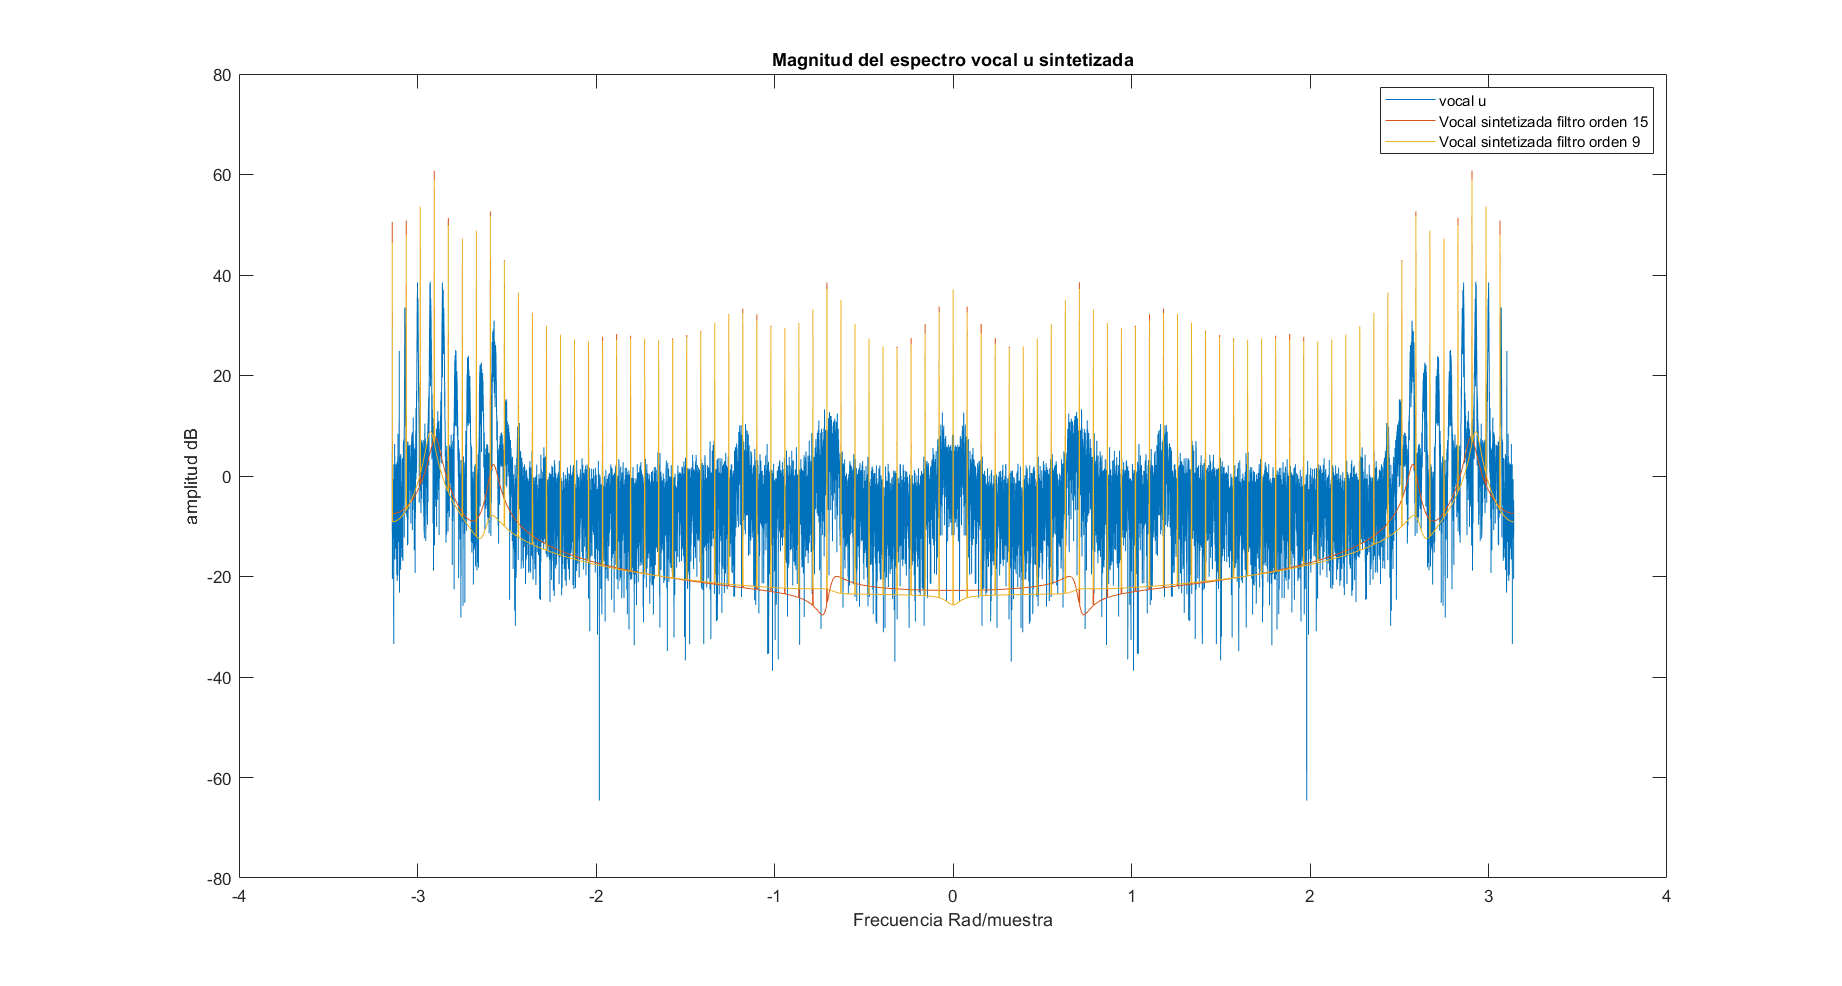
\includegraphics[width = 0.9 \linewidth]{Figuras/P4_3M_u.png}
    \caption{Magnitud de la vocal 'u' original y sintetizada.}
    \label{P4_3M_u}
\end{figure}
%
\begin{figure}[H]
    \centering
    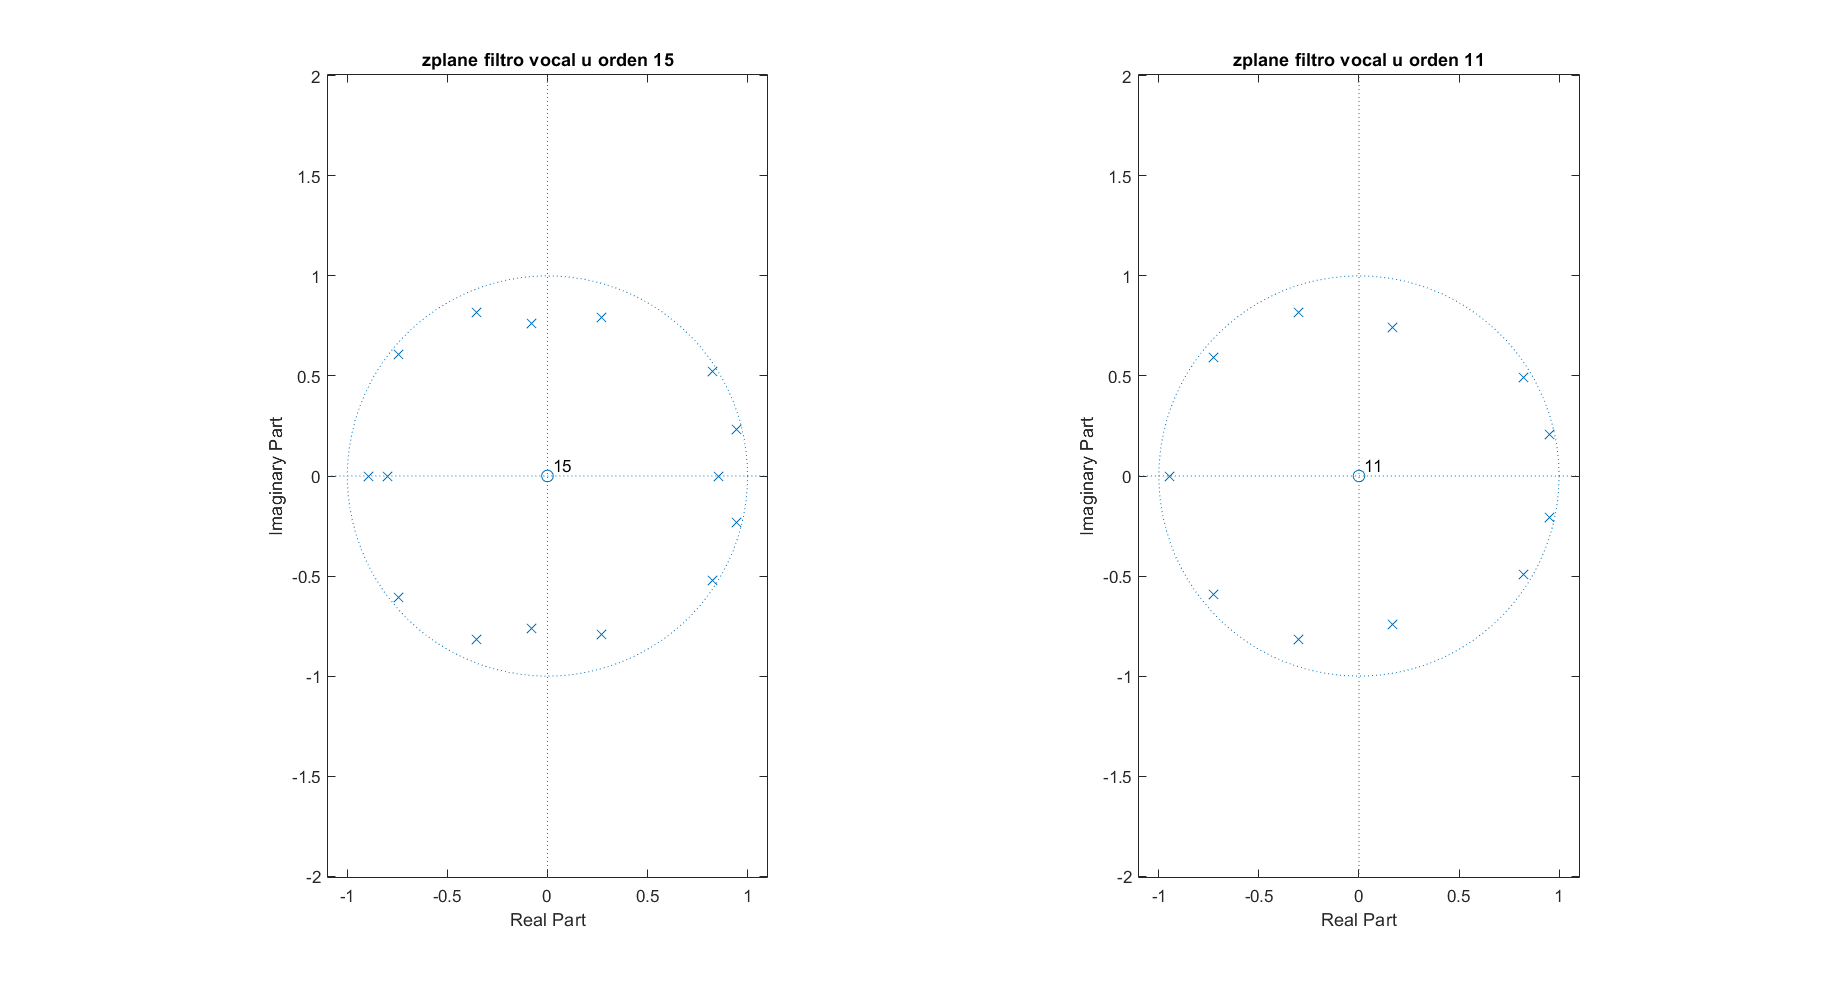
\includegraphics[width = 0.9 \linewidth]{Figuras/P4_3Z.png}
    \caption{Planos Z de vocal 'u' para distintos ordenes.}
    \label{P4_3Z_u}
\end{figure}

Una estrategia para determinar el orden de un filtro AR para LPC es obtener el espectro positivo de la señal a sintetizar. Observar el número $n$ de formantes (sin incluir la frecuencia $0$). Multiplicar el número por $2$ para obtener $n$ pares de polos complejos conjugados, y agregar un polo en $0$. Por lo tanto el orden debe ser de $2n+1$. \\

%
\item %4)------------------------------------------------------------------% 
%

\begin{itemize}
    \item 
    El comando \texttt{tfsos} de matlab obtiene los coeficientes de los $n/2$ filtros biquad que al conectarse en cascada, entregan la función de transferencia de orden $n$ ingresada. En el caso que $n$ sea impar, el comando entregará además el filtro de orden $1$ restante.
    
    Las filas de la matriz \texttt{sos} corresponden a cada filtro biquad cuyos coeficientes están dados por las columnas. Por lo tanto la matriz siempre tendrá $5$ columnas mientras que el número de filas depende del orden de la función de transferencia ingresada.
    
    La variable entregada \texttt{g} corresponde a la ganancia por la cual multiplicar los filtros biquad para obtener la transferencia deseada. 
    \item
    Se utilizó el comando \texttt{tfsos} para obtener los filtros biquad que obtienen el filtro lpc de orden $15$ para la vocal \textit{a} en cascada. En este caso se utilizarán los $7$ filtros biquad, ignorando el filtro de orden $1$ restante.

    La magnitud de la vocal 'a' con los diferentes filtros biquad se presenta en la Figura \ref{P4_3}. Donde se observa que cada filtro tiene polos complejos conjugados correspondientes a la frecuencia de una de las formandes de la vocal.
%
\begin{figure}[H]
    \centering
    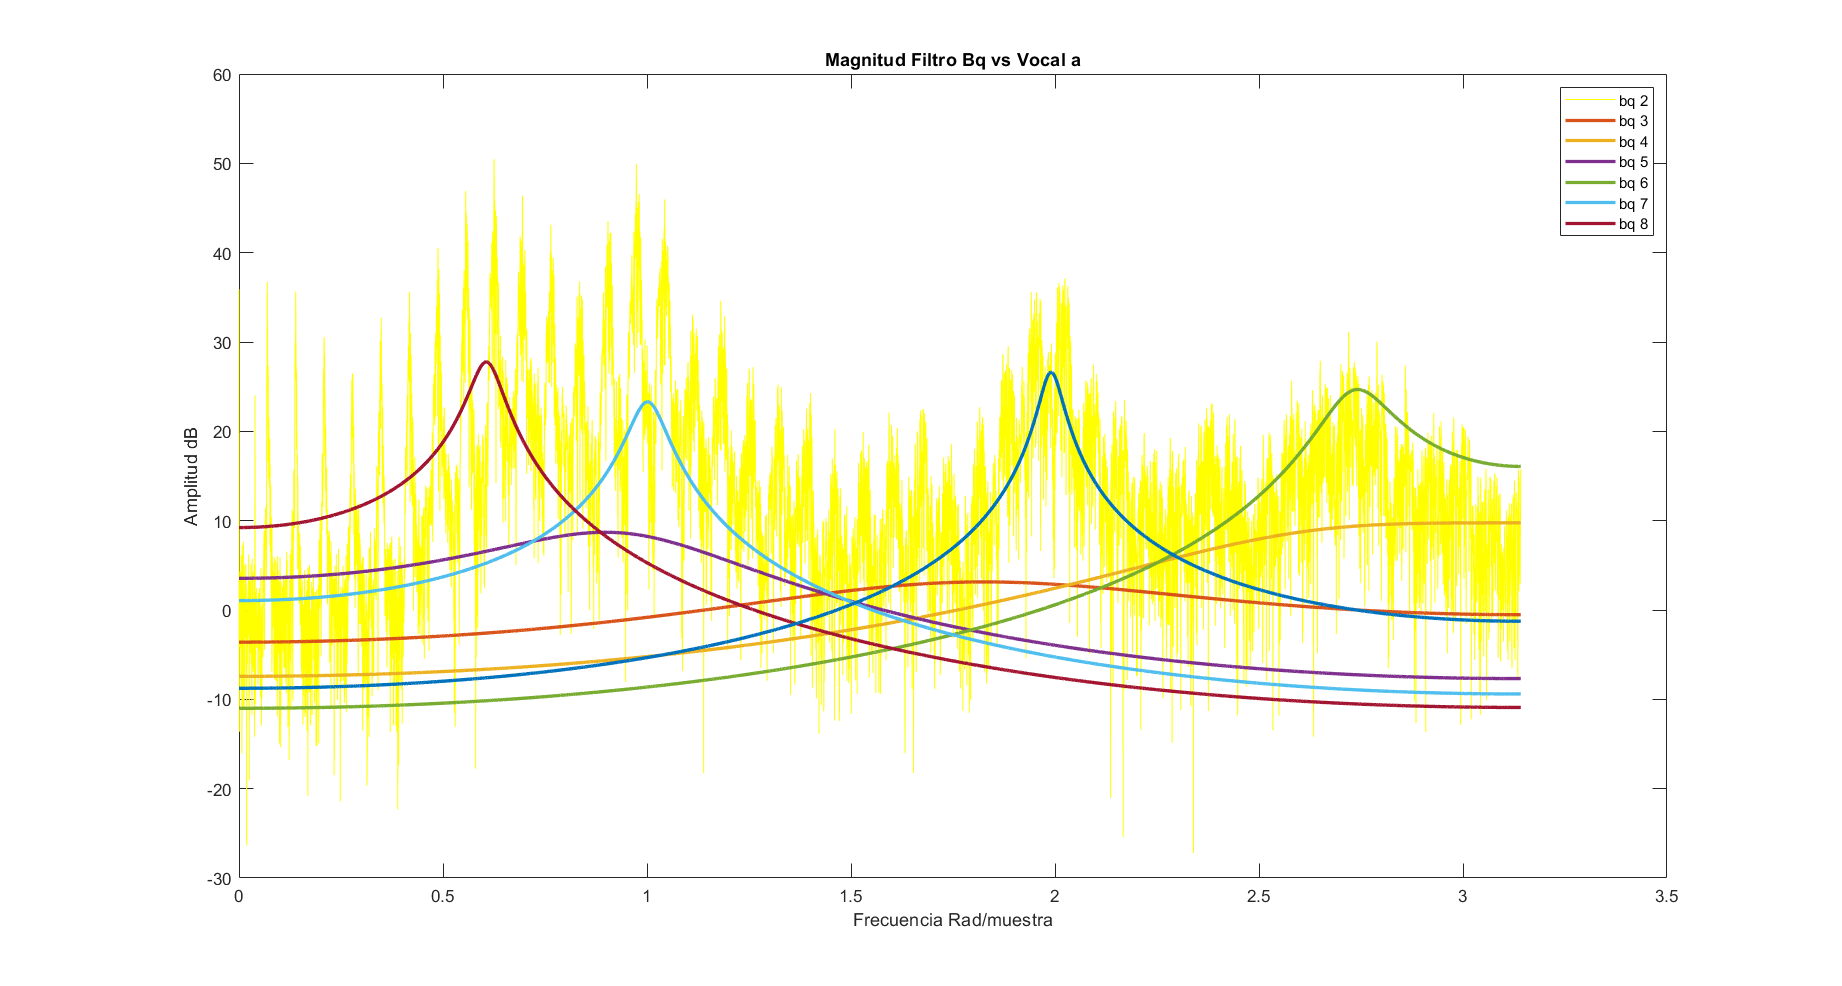
\includegraphics[width = 0.9 \linewidth]{Figuras/P4_3.png}
    \caption{Magnitud de la vocal 'a' y diferentes filtros bq.}
    \label{P4_3}
\end{figure}
\end{itemize}
\end{enumerate}
%%%%%%%%%%%%%%%%%%%%%%%%%%%%%%%%%%%%%%%%%%%%%%%%%%%%%%%%%%%%%%%%%%%%%%%%%%%%%%%%%
%
%--V.OBSERVANDO EL RESIDUO DE PREDICCION------------------------%
%
%%%%%%%%%%%%%%%%%%%%%%%%%%%%%%%%%%%%%%%%%%%%%%%%%%%%%%%%%%%%%%%%%%%%%%%%%%%%%%%%%
\section{Observando el residuo de predicción}
\begin{enumerate}[1)]
\item %1)------------------------------------------------------------------% 
%
La respuesta en frecuencia del filtro inverso vs el filtro AR de orden 15 se muestra en la Figura \ref{P5_1}.
%
\begin{figure}[H]
    \centering
    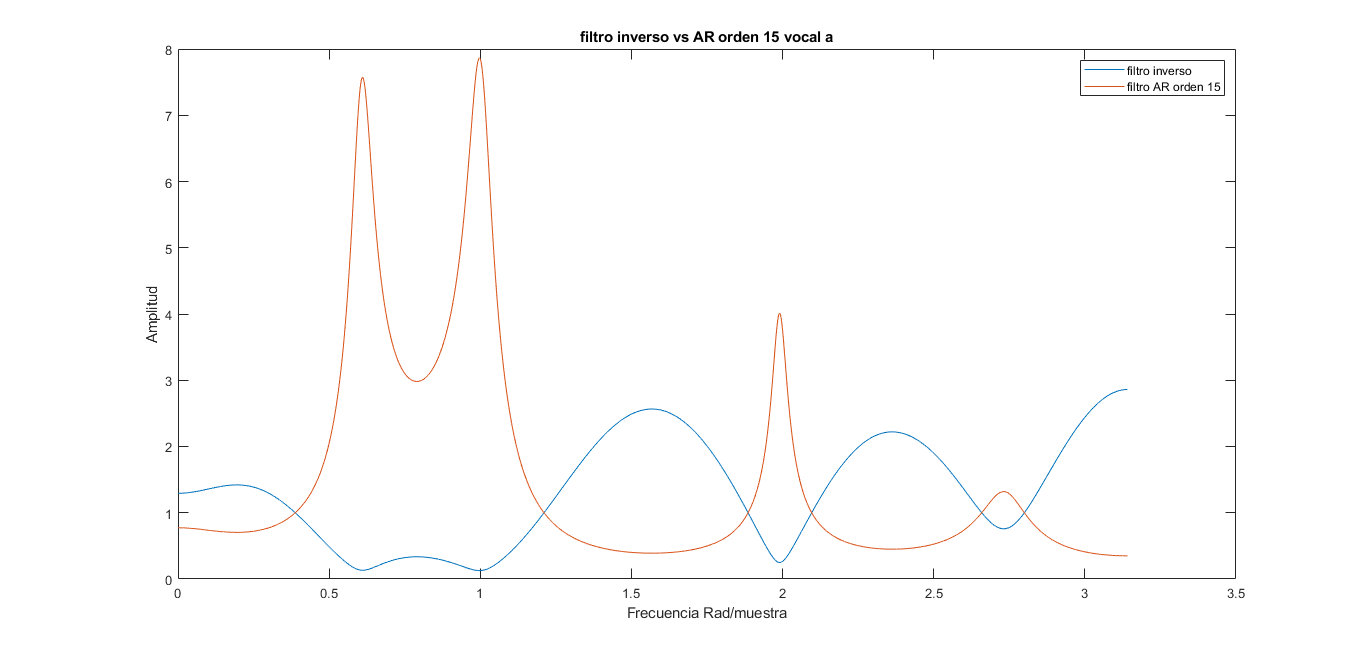
\includegraphics[width = 0.9 \linewidth]{Figuras/P5_1.png}
    \caption{Filtro AR vd filtro inverso.}
    \label{P5_1}
\end{figure}
%
\item %2)------------------------------------------------------------------% 
%
Se obtiene el residuo luego de aplicar el filtro inverso a la vocal \textit{a}.

El gráfico del residuo se presenta en Figura \ref{P5_2}. Se observa que este se asemeja bastante a un tren de impulsos, por lo que este resulta una aproximación adecuada. Sin embargo la señal no es exactamente igual a un tren, habiendo otros componentes entre los peaks, cuya inclusión podría mejorar la verosimilitud de las señales sintetizadas..
%
\begin{figure}[H]
    \centering
    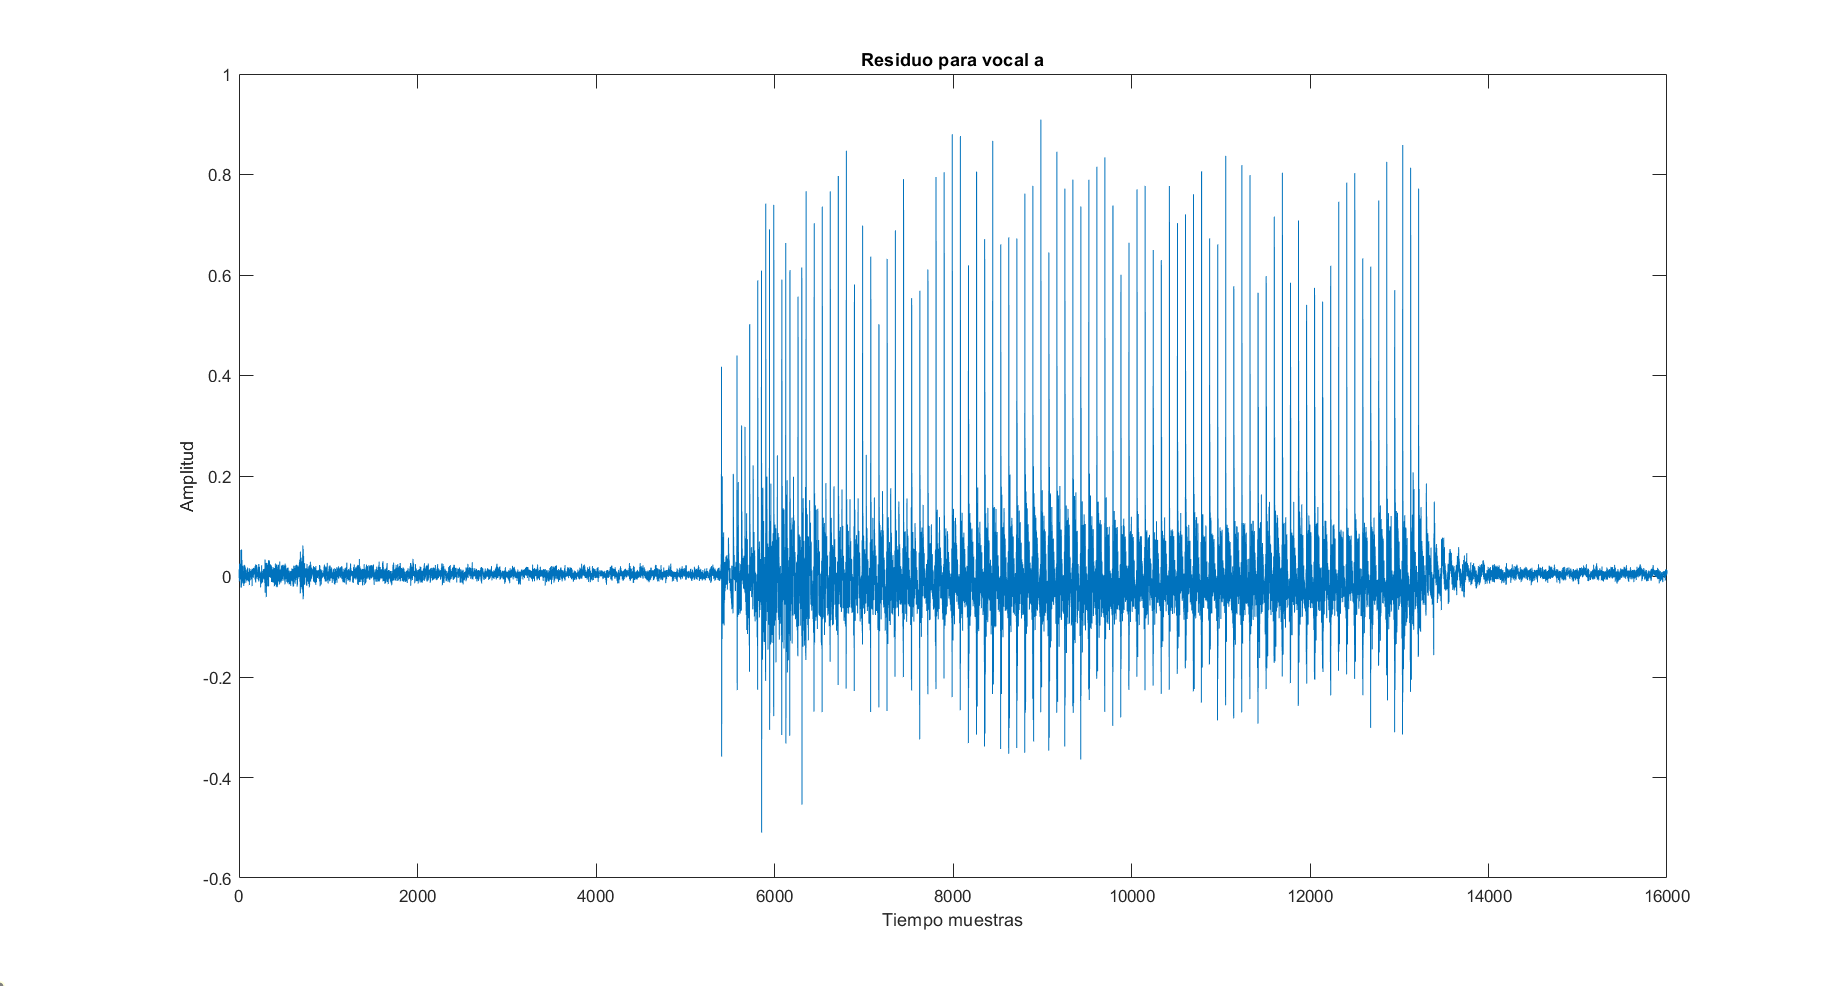
\includegraphics[width = 0.9 \linewidth]{Figuras/P5_2.png}
    \caption{Residuo de la señal vocal 'a'.}
    \label{P5_2}
\end{figure}
%
\item %3)------------------------------------------------------------------% 
%
El espectro en frecuencia del residuo de la vocal 'a' y de la señal vocal 'a' se presentan en Figura \ref{P5_3}. Se observa que la mayoría del componente armónico de la señal es eliminada por el filtro inverso al obtener el residuo. Sin embargo, el espectro del residuo no es completamente plano, habiendo componentes mayores en frecuencias más bajas.

Se observa también que el ruido es más significativo en el residuo que en la vocal.
%
\begin{figure}[H]
    \centering
    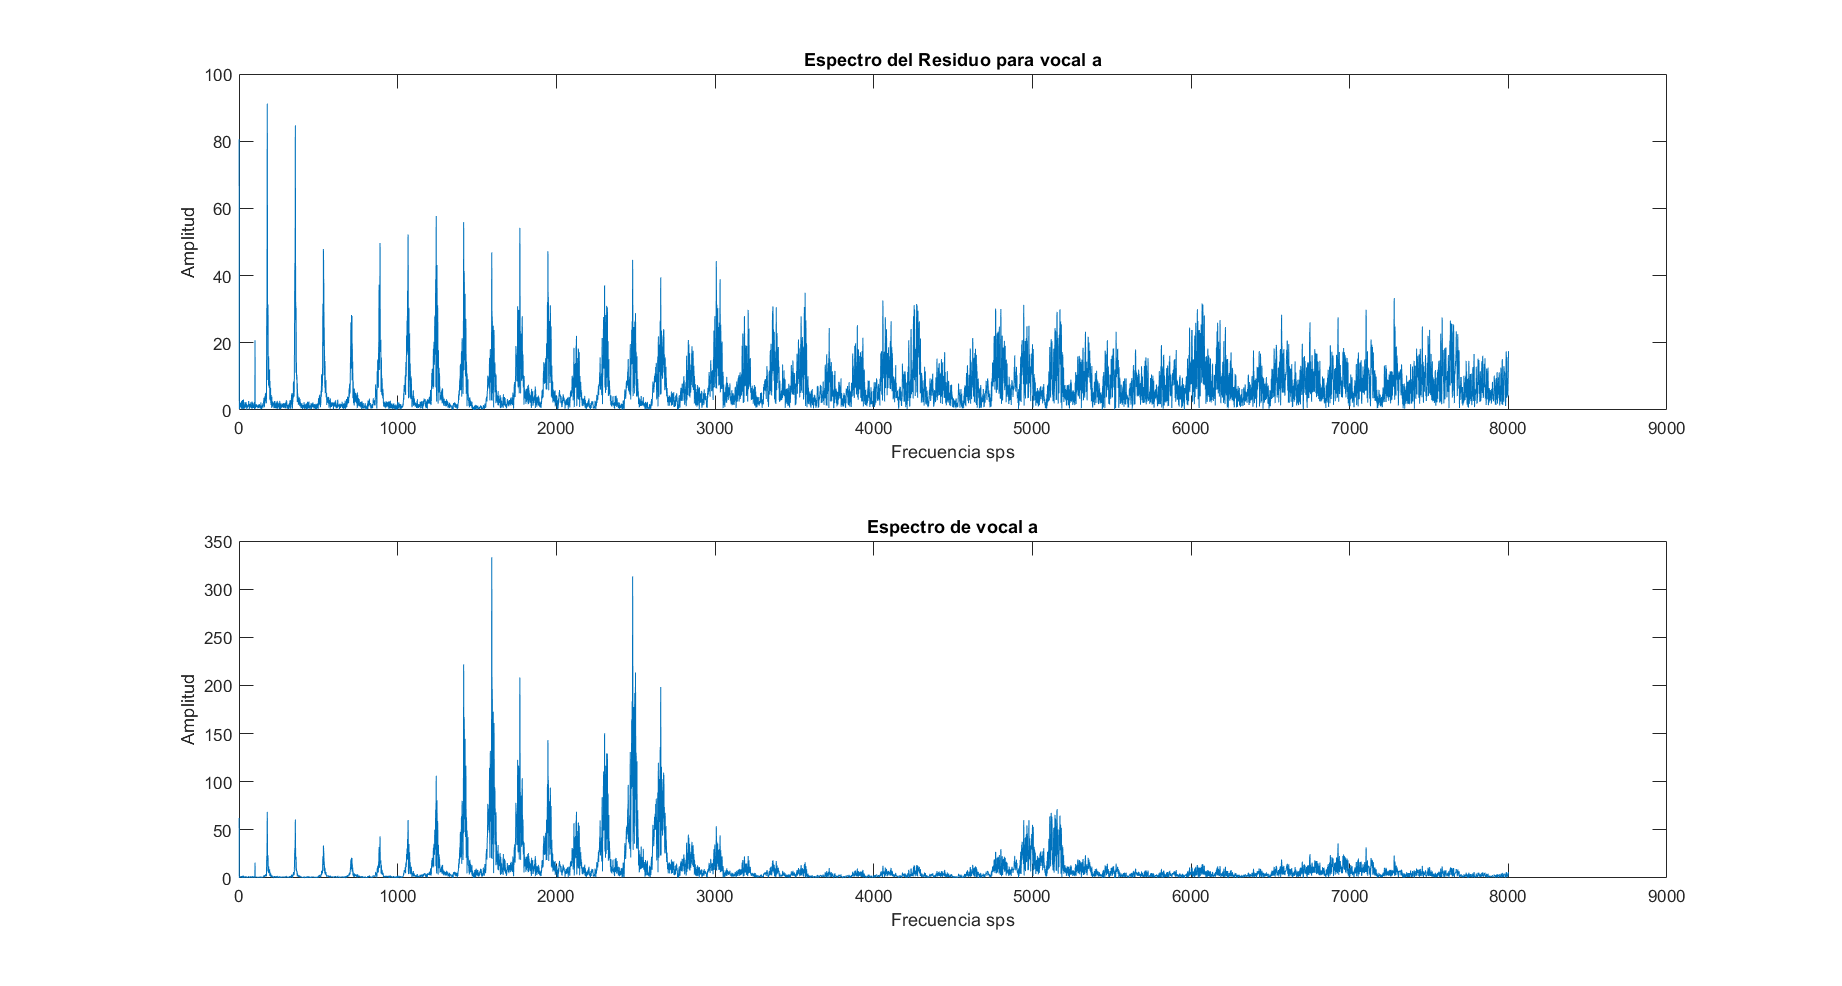
\includegraphics[width = 0.9 \linewidth]{Figuras/P5_3.png}
    \caption{Residuo de la señal vocal 'a'.}
    \label{P5_3}
\end{figure}
%
\item %4)------------------------------------------------------------------% 
%
La autocorrelación del residuo y de la vocal se muestran en la Figura \ref{P5_4}.

Se observa que la frecuencia fundamental es obtenida muy facilmente de la autocorrelación del residuo de la señal. 

En particular, para señales que no son solamente una vocal sostenida, los componentes entre frecuencias puede hacer confusa la obtención de las frecuencias, estos prácticamente desaparecen al calcular la correlación del residuo, por lo que el uso de esta simplificaría mucho más la obtención de la fundamental.
%
\begin{figure}[H]
    \centering
    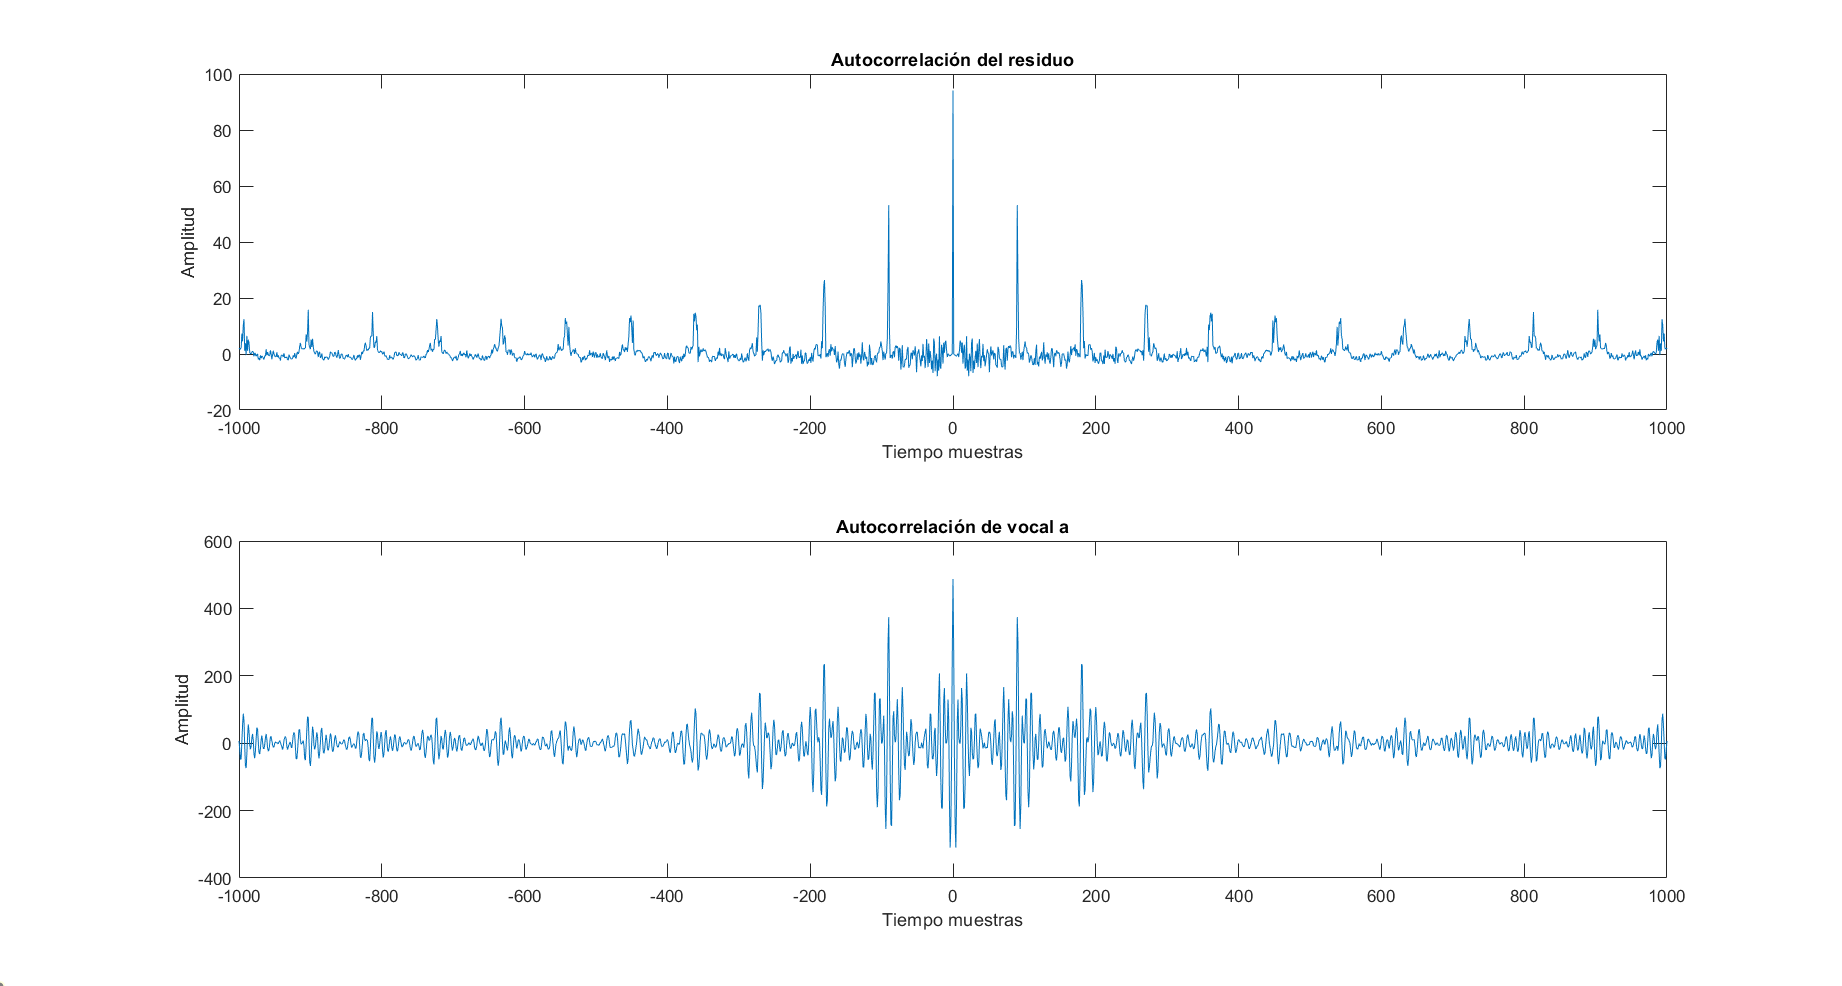
\includegraphics[width = 0.9 \linewidth]{Figuras/P5_4.png}
    \caption{Autocorrelación entre residuo y vocal.}
    \label{P5_4}
\end{figure}
%
\end{enumerate}
\end{document}
